%%%%%%%%%%%%%%%%%%%%%%%%%%%%%%%%%%%%%%%%%%%%%%%%%%%%%%%%%%%%%%%%%%%%%%%%%%%%%%%%
\documentclass[11pt]{report}
%%%%%%%%%%%%%%%%%%%%%%%%%%%%%%%%%%%%%%%%%%%%%%%%%%%%%%%%%%%%%%%%%%%%%%%%%%%%%%%%
% PDF output?
\newif\ifpdf
\ifx\pdfoutput\undefined
  \pdffalse
\else
  \pdfoutput=1
  \pdftrue
\fi
%%%%%%%%%%%%%%%%%%%%%%%%%%%%%%%%%%%%%%%%%%%%%%%%%%%%%%%%%%%%%%%%%%%%%%%%%%%%%%%%
\usepackage{graphicx}
\usepackage{algorithmic}
\usepackage{float}
\usepackage{subfigure}
\setlength{\parindent}{0pt}
\ifpdf
  \RequirePackage[pdftex, colorlinks=true, pdfstartview=FitH, linkcolor=blue, citecolor=blue, urlcolor=blue]{hyperref}
  \pdfinfo{
  /Title    (Verdict Library Reference Manual)
  /Author   (C. J. Stimpson, C. D. Ernst, P. Knupp, P. P. Pebay, and D. Thompson)
  /Keywords ()
  }
\else
  \RequirePackage{hyperref}
\fi
% ----------------------------------------------------------------------
% -- Packages
% ----------------------------------------------------------------------
\RequirePackage{amsthm}
\RequirePackage{amsbsy,amsmath}
\RequirePackage{amsfonts,amssymb}
% ----------------------------------------------------------------------
% -- Mathematical environment
% ----------------------------------------------------------------------
% -- theorems & related topics
\theoremstyle{plain}
\newtheorem{theo}{Theorem}[section]
\newtheorem{prop}[theo]{Proposition}
\newtheorem{lemm}[theo]{Lemma}
\newtheorem{coro}[theo]{Corollary}
% -- definitions & examples
\theoremstyle{definition}
\newtheorem{defi}{Definition}[section]
\newtheorem{axio}{Axiom}[section]
% -- remarks & axioms
\theoremstyle{remark}
\newtheorem{rema}{Remark}[section]
\newtheorem{exam}{Example}[section]
% -- algorithms
\newtheoremstyle{algostyle}% name
  {}%      Space above, empty = `usual value' 
  {}%      Space below
  {}%         Body font
  {}%         Indent amount (empty = no indent, \parindent = para indent)
  {\bfseries}% Thm head font
  {}%        Punctuation after thm head
  {\newline}% Space after thm head: \newline = linebreak
  {\thmname{#1}\thmnumber{ #2.}{ \texttt{[#3]}}}% Thm head spec
\theoremstyle{algostyle}
\newtheorem{algo}{Algorithm}
% ----------------------------------------------------------------------
% -- Mathematical macros
% ----------------------------------------------------------------------
% -- N, Z, R & C
\newcommand{\N}{\rm I\kern-.16em N}
\newcommand{\Z}{\mathchoice{\sf\textstyle Z\kern-0.4em Z}
{\sf\textstyle Z\kern-0.4em Z}
{\sf\scriptstyle Z\kern-0.3em Z}
{\sf\scriptscriptstyle Z\kern-0.2em Z}}
\newcommand{\R}{\rm I\kern-.16em R}
\newcommand{\C}{\mathchoice{\setbox0=\hbox{$\displaystyle\rm C$}%
\hbox{\hbox to0pt{\kern0.4\wd0\vrule height0.9\ht0\hss}\box0}}
{\setbox0=\hbox{$\textstyle\rm C$}\hbox{\hbox
to0pt{\kern0.4\wd0\vrule height0.9\ht0\hss}\box0}}
{\setbox0=\hbox{$\scriptstyle\rm C$}\hbox{\hbox
to0pt{\kern0.4\wd0\vrule height0.9\ht0\hss}\box0}}
{\setbox0=\hbox{$\scriptscriptstyle\rm C$}\hbox{\hbox
to0pt{\kern0.4\wd0\vrule height0.9\ht0\hss}\box0}}}
% -- differential calculus
\providecommand{\diff}[2]{\frac{\partial {#1}}{\partial {#2}}}
\providecommand{\ddiff}[2]{\frac{\partial^2 {#1}}{\partial {#2}^2}}
\providecommand{\dtiff}[3]{\frac{\partial^2 {#1}}{\partial {#2} \partial {#3}}}
% -- integral calculus
\providecommand{\sint}[4]{\int_{#1}^{#2}{#3}\,\mathrm{d}{#4}}
\providecommand{\dint}[3]{\iint_{#1}{#2}\,\mathrm{d}{#3}}
\providecommand{\tint}[3]{\iiint_{#1}{#2}\,\mathrm{d}{#3}}
% -- vector calculus
\providecommand{\ve}[1]{\overrightarrow{#1}}
\providecommand{\norm}[1]{\left\lVert{#1}\right\rVert}
\providecommand{\normsup}[1]{\norm{#1}_\infty}
\providecommand{\scalprod}[2]{\langle{#1},{#2}\rangle}
%%%%%%%%%%%%%%%%%%%%%%%%%%%%%%%%%%%%%%%%%%%%%%%%%%%%%%%%%%%%%%%%%%%%%%%

%%%%%%%%%%%%%%%%%%%%%%%%%%%%%%%%%%%
\graphicspath{{.}{./png/}{./svg/}}
%%%%%%%%%%%%%%%%%%%%%%%%%%%%%%%%%%%
\newcommand{\Sf}{\mathfrak{S}_4}
\newcommand{\verd}{\textsf{Verdict}}
\newcommand{\cubit}{\textsf{CUBIT}}
\newcommand{\verde}{\textsf{VERDE}}
\newcommand{\vtk}{\textsf{VTK}}
\newcommand{\PV}{\textsf{ParaView}}
\newcommand{\nsup}{\textrm{Not supported}}
\newcommand{\dgr}{\ensuremath{^{\circ}}}
\newcommand{\normvec}[1]{\big\lVert{\vec#1}\big\rVert}
%%%%%%%%%%%%%%%%%%%%%%%%%%%%%%%%%%%
\title{The \verd{} Library Reference Manual}
\author{C. J. Stimpson\\
        Elemental Technologies, Inc.\\
        17 N. Merchant St.\\
        American Fork, UT 84003, U.S.A.\\
        \texttt{clinton@elemtech.com}
        \and
        C. D. Ernst\\
        Elemental Technologies, Inc.\\
        17 N. Merchant St.\\
        American Fork, UT 84003, U.S.A.\\
        \texttt{corey@elemtech.com}
        \and
        P. Knupp\\
        Sandia National Laboratories\\
        M.S. 1318, P.O. Box 5800\\
        Albuquerque, NM 87185, U.S.A.\\
        \texttt{pknupp@sandia.gov}
        \and
        P. P. P\'ebay\\
        Sandia National Laboratories\\
        M.S. 9051, P.O. Box 969\\
        Livermore, CA 94550, U.S.A.\\
        \texttt{pppebay@sandia.gov}
        \and
        D. Thompson\\
        Sandia National Laboratories\\
        M.S. 9152, P.O. Box 969\\
        Livermore, CA 94550, U.S.A.\\
        \texttt{dcthomp@sandia.gov}
}
\date{April 2007}
%%%%%%%%%%%%%%%%%%%%%%%%%%%%%%%%%%%%%%%%%%%%%%%%%%%%%%%%%%%%%%%%%%%%%%%%%%%%%%%%
\begin{document}
%%%%%%%%%%%%%%%%%%%%%%%%%%%%%%%%%%%%%%%%%%%%%%%%%%%%%%%%%%%%%%%%%%%%%%%%%%%%%%%%
\maketitle
%%%%%%%%%%%%%%%%%%%%%%%%%%%%%%%%%%%
\begin{abstract}
\verd\ is a collection of subroutines for evaluating the geometric qualities
of triangles, quadrilaterals, tetrahedra, and hexahedra using a variety of
metrics.
A metric is a real number assigned to one of these shapes depending on its
particular vertex coordinates.
These metrics are used to evaluate the input to finite element, finite volume,
boundary element, and other types of solvers that approximate the solution to
partial differential equations defined over regions of space.
The geometric qualities of these regions is usually strongly tied to the
accuracy these solvers are able to obtain in their approximations.

The subroutines are written in C++ and have a simple C interface.
Each metric may be evaluated individually or in combination.
When multiple metrics are evaluated at once, they share common
calculations to lower the cost of the evaluation.
\end{abstract}
%%%%%%%%%%%%%%%%%%%%%%%%%%%%%%%%%%%
\clearpage
\section*{Acknowledgements}
The authors would like to acknowledge, in no particular order, the
following individuals:
Jason Shepherd, Robert Kerr, Rob Leland, Tim Tautges, Ray Meyers, Karl
Merkley, Greg Sjaardema, David White, and Scott Mitchell.\\

Authors affiliated with Sandia National Laboratories were supported by
the United States Department of Energy, Office of Defense
Programs. Sandia is a multiprogram laboratory operated by Sandia
Corporation, a Lockheed-Martin Company, for the United States
Department of Energy under contract DE-AC04-94-AL85000.
%%%%%%%%%%%%%%%%%%%%%%%%%%%%%%%%%%%
\clearpage
\tableofcontents
\listoffigures
%\listoftables
\cleardoublepage
%%%%%%%%%%%%%%%%%%%%%%%%%%%%%%%%%%%
\chapter{Introduction}

This is \verd, a library for evaluating the geometric qualities of regions of space.
These regions of space are typically those used as problem domains for partial differential equations,
and are typically partitioned into subregions known as finite elements, finite volumes, or boundary elements.
Subregions are typically simple shapes defined by a few vertices.
The subregion shapes \verd\ currently supports include triangles, quadrilaterals, tetrahedra, and hexahedra.

\section{Measuring Quality with Metrics}

\verd\ evaluates geometric qualities on a subregion of the partition with metrics.
A metric is a real number that may be assigned to the subregion.
Some metrics, which we will call \textbf{proper metrics}, are normalized so that
their values are $1$ for ideally-shaped subregions and
their values tend to $\infty$ for ill-defined, poor quality, or degenerate subregions.
Examples where a proper metric should tend to $\infty$ include non-planar quadrilaterals,
triangles with edges of vastly different lengths, and subregions with coincident vertices.

\section{History of \verd}

\verd\ has its first roots in the \href{http://www.cs.sandia.gov/capabilities/VerdeMeshVerificationSuite/index.html}{\verde}\footnote{\href{http://www.cs.sandia.gov/capabilities/VerdeMeshVerificationSuite/index.html}%
           {\texttt{http://www.cs.sandia.gov/capabilities/VerdeMeshVerificationSuite/index.html}}} project.
\verde\ is a simple program to
read Exodus meshes, and analyze them for possible problems.  Quality was one of
the areas of analysis that \verde\ covers.  It was realized that \verde\  and 
\href{http://cubit.sandia.gov/}{\cubit}\footnote{\href{http://cubit.sandia.gov/}{\texttt{http://cubit.sandia.gov/}}} did not yield the same results when analyzing the geometric qualities of meshes.
As a result, \verd\ was created so that both \verde\ and \cubit\ could share the same
code and produce the same results.  \verd\ also has roots in the \cubit\ project
and many other contributors, both theoretical and practical.
\verd\ was initially licensed under the LGPL.

Meanwhile, the \href{http://www.vtk.org/}{Visualization Tool Kit
(\vtk)\footnote{\href{http://www.vtk.org/}{\texttt{http://www.vtk.org/}}}} did not 
have any support for general purpose mesh quality assessment (with the
exception of a method to calculate the tetrahedral radius ratio,
written by Leila Baghdadi, Hanif Ladak, and David Steinman at the
Imaging Research Labs, Robarts Research Institute). Due to the need for
such a tool, and because Kitware was unwilling at that time to
include LGPL libraries in the \vtk\ repository, Philippe
P\'ebay and David Thompson generalized the \href{http://www.vtk.org/doc/nightly/html/classvtkMeshQuality.html}{\texttt{vtkMeshQuality}}\footnote{\href{http://www.vtk.org/doc/nightly/html/classvtkMeshQuality.html}%
                 {\texttt{http://www.vtk.org/doc/nightly/html/classvtkMeshQuality.html}}}
filter in 2004 to compute one or more measures of geometric quality for each 2-D
and 3-D cell (triangle, quadrilateral, tetrahedron, or hexahedron) of
a mesh for a variety of metrics.
In addition to computing per-element qualities, methods to compute their average, minimum, maximum,
and variance over the entire mesh where also added.
These descriptive statistics are stored in the output mesh's \textsc{FieldData}. This filter allows forx
further processing and/or visualization of the per-element quality,
for instance using
\href{http://www.paraview.org/}{\PV\footnote{\href{http://www.vtk.org/}{\texttt{http://www.paraview.org/}}}}
as illustrated in Figure~\ref{f:viz-qual}
%%%%%%%%%%%%%%%%%%%%%%%%%%%%%%%%%%%%
\begin{figure}[ht]
\begin{center}
\hfil
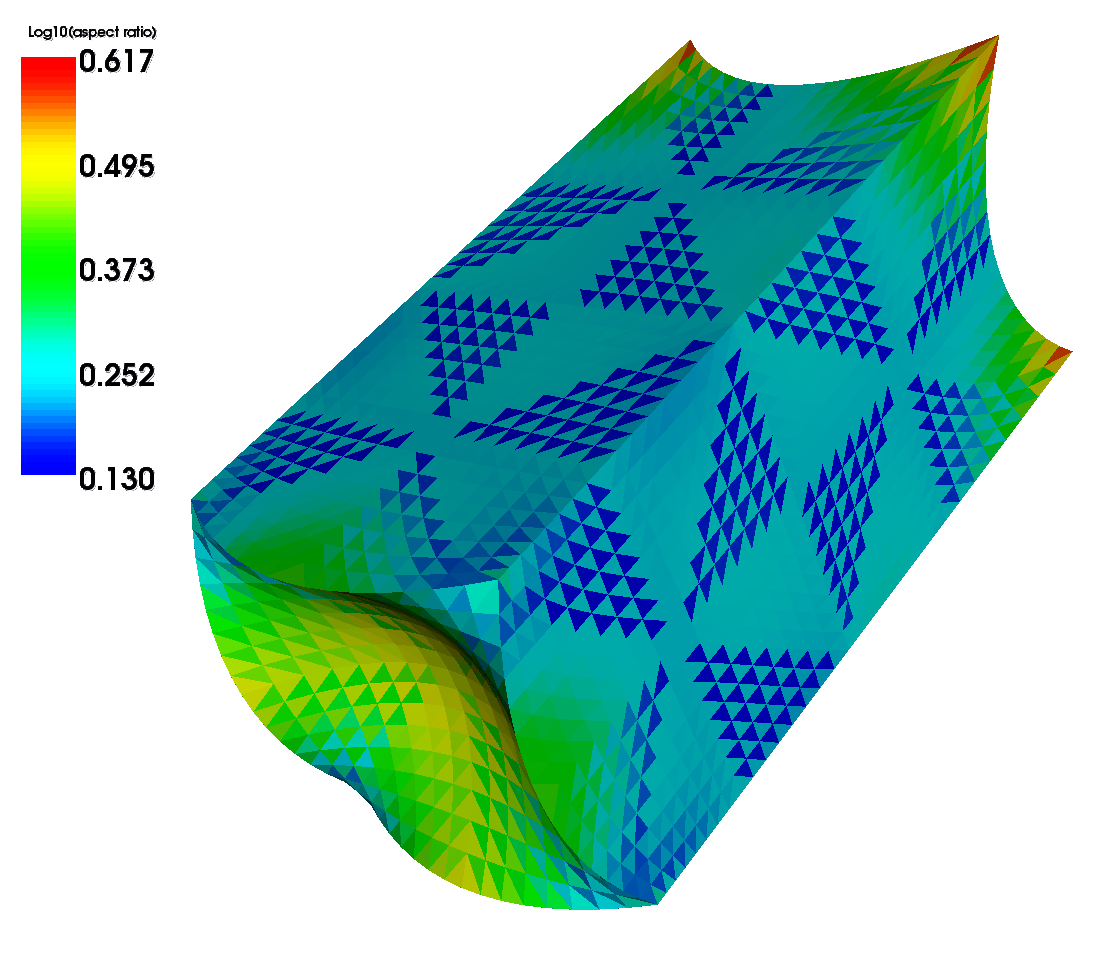
\includegraphics[height=4.5cm]{quality-streamingTess}
\hfil
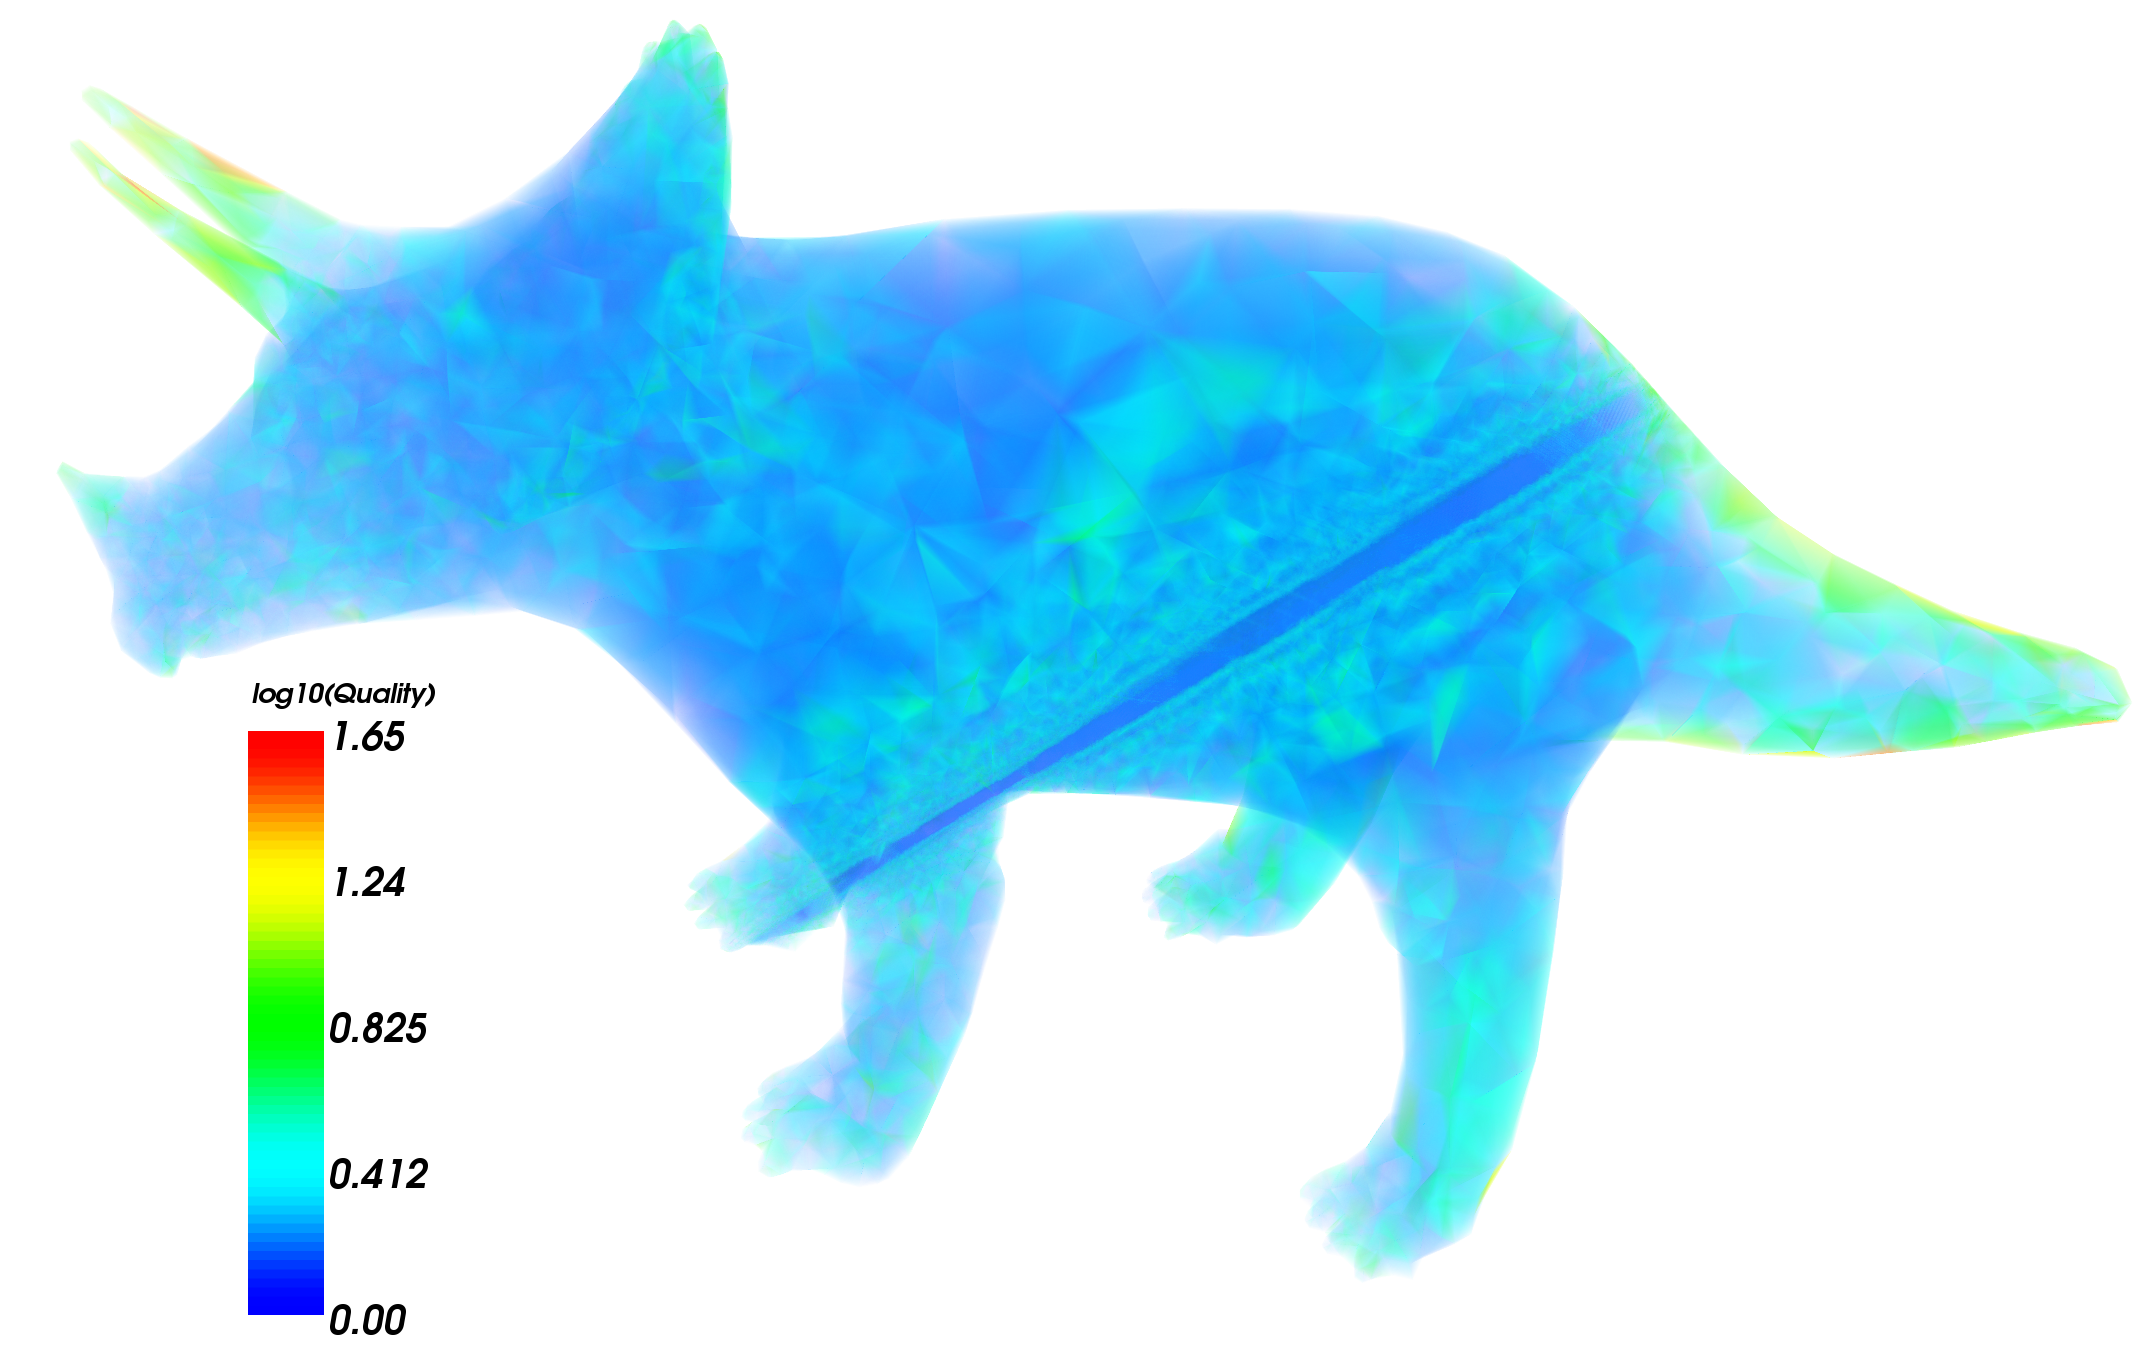
\includegraphics[height=4.5cm]{tri4qualVR-bq2}
\hfil
\caption{\label{f:viz-qual} Surface (left) and volume (right)
renderings with \PV\ of the per-element base-$10$ logarithms of the
aspect ratios for two tetrahedral meshes.} 
\end{center}
\end{figure}
%%%%%%%%%%%%%%%%%%%%%%%%%%%%%%%%%%%%

Following a change in \verd's licensing scheme, from the LGPL to a modified BSD-style license,
it was decided in late 2006 to use \verd\ in \vtk\ for the same reasons that \verd\ was initially
created, by:
\begin{enumerate}
\item 
moving all metric implementations from \texttt{vtkMeshQuality} to
\verd\, while retaining the best implementation when the same metric
was implemented in both software packages;
\item
using \texttt{vtkMeshQuality} as a wrapper around \verd{}; and
\item
\label{item:API-changes}
resolving naming inconsistencies and redundancies.
\end{enumerate}
It is important to former \verd\ users to note that
item~\ref{item:API-changes} has resulted in changes to \verd{}s API,
although efforts have been made to preserve backwards-compatibility
as often as possible; this document underscores these modifications.

\section{Organization}

After this introduction, the document can be broadly divided into sections covering
first the practical aspects and
second the theoretical aspects of geometric quality evaluation.
In these sections:
\begin{itemize}
\item Instructions on the practical aspects of obtaining, building, and installing the library are described.
\item Notes on the application programming interface (API) are provided.
\item A summary of each metric is provided, sorted first by the shape of the subregion they deal with and then by name.
\end{itemize}

The summaries in the last section form the bulk of the document and
each contains a mathematical description of its quality metric $q$.
In addition to a formula for each metric, information on the typical, acceptable, and total range
of values taken on are presented in a tabular form according to the conventions outlined below in \S\ref{s:metric-range}.
Each summary table also contains a note on the dimension of its metric -- where we use
dimension in terms of the units associated with each metric value.
Proper metrics have no dimension (which is denoted with a $1$) but some metrics
such as area, volume, or maximum angle do have dimension.
We use $L$ to denote dimensions of length and $A$ to denote dimensions of angle.
When a metric has a dimension repeated, an exponent is used to show the count.
For example, volume has 3 length dimensions and would be denoted $L^3$.
While the precise units of length depend on the input coordinates,
angles are always reported in degrees.
The summary table also contains an entry for the value that the metric takes on for some
ideally-shaped subregion, when the metric is shape-invariant (unlike,
\emph{e.g.} volume metrics which are not preserved by scaling). For
triangular, quadrilateral, tetrahedral, and hexahedral shapes, this is
respectively an equilateral triangle, a square, a regular tetrahedron,
and a cube. For proper metrics, this value will be $q = 1$.
Finally, each summary table has a reference to a book or paper where its metric is defined and discussed.
If no reference is listed, the metric is one that is traditionally used but not present
in the literature we are aware of.

Where possible, notes on the intended use of the metric are included.
\verd\ provides a variety of metrics for each subregion shape it supports.
Since a metric is a single real number, it cannot completely describe the shape of its corresponding subregion.
Thus, most metrics are used to identify a single type of problem with a subregion's shape.
Because many numerical techniques are used to solve partial differential equations,
the best metric to characterize the geometric quality of a region will vary.

\section{Metric Ranges\label{s:metric-range}}

Each metric may take on any value on the real number line, but typically subsets of this range
are of interest since values for misbehaved or geometrically degenerate elements are often used to
segregate or eliminate elements.
The summary tables provided for each metric include three intervals on the real number line:
\begin{center}
\begin{tabular}{r@{ : }p{3.2in}}\hline
Acceptable Range&Well-behaved elements will have metrics in this range.\\
Normal Range    &All elements except those with degeneracies will have metrics in this range.\\
Full Range      &All elements including degenerate ones will have metrics in this range.\\ \hline
\end{tabular}
\end{center}

\section{Metric Behavior}

The metrics in this report are all checked for overflow like so:
\begin{algorithmic}[1]
\STATE Given a double-precision quality metric value $q$,
\IF{$q > 0$}
\STATE $q\gets\min\left( q, DBL\_MAX \right)$
\ELSE
\STATE $q\gets\max\left( q, -DBL\_MAX \right)$
\ENDIF
\end{algorithmic}

Where applicable, the metrics in \verd\ were verified against theory for:
\begin{itemize}
\item Node order invariance.
\item Continous solutions within the normal range.
\end{itemize}

\cleardoublepage
%%%%%%%%%%%%%%%%%%%%%%%%%%%%%%%%%%%
\chapter{Obtain, Configure, Compile, Install}

The \verd\ repository now resides at Kitware, Inc. and is publicly available.
A formal release has not yet been made since the repository has been moved and
so you will need to obtain \verd\ source code from CVS.
If you intend to build \vtk,
you need not obtain or compile \verd\ separately since it is included with VTK.

\section{Prerequisites}

To build \verd\ you will need a C++ compiler.
GNU's gcc 3 or above, Intel's icc 8 or above, Apple's Xcode 2.4 or above,
Borland's bcc 3.2 or 5.5, and Microsoft's VC 6 or above are all known to work.
Other compilers, including Sun's CC, DEC's cxx, IBM's xlC, HP's aCC, and SGI's CC, are untested but should work.
Unless you are using Microsoft's Visual Studio compilers, you will also need ``make''.

It is not required, but \href{http://www.cmake.org/}{CMake}\footnote{\texttt{\href{http://www.cmake.org}{http://www.cmake.org}}}
version 2.4 or above is highly recommended.
At some point in the future, this will be the only supported configuration system.

\section{Obtaining \verd}

Fetch the source code from Kitware's CVS server at \texttt{www.vtk.org}.
Kitware provides anonymous access using CVS pserver.
Before you can retrieve the source code, you must authenticate yourself to the CVS server.
From a terminal window, run
\begin{verbatim}
    cvs -d :pserver:anonymous@www.vtk.org:/cvsroot/VTK login
\end{verbatim}
You will be prompted for a password. Use ``vtk'' (without the quotes).
You may then retrieve \verd\ by running
\begin{verbatim}
    cvs -d :pserver:anonymous@www.vtk.org:/cvsroot/VTK -z3 \
        co -d Verdict VTK/Utilities/verdict
\end{verbatim}
This will place the source code in a subdirectory named \texttt{Verdict}.

If the machine you will use to compile \verd\ is behind a firewall,
you will probably not be able to use the commands above to obtain the source code.
If you have SSH access to a computer that is not behind a firewall and
SSH port forwarding is not forbidden, you may port forward CVS requests using a pair of
terminal windows.
For the purposes of our description,
say that you will build \verd\ on a computer named \texttt{inside.thefirewall.com} (behind the firewall) and
have SSH access to a computer named \texttt{outside.thefirewall.com} (which is not behind the firewall).

In the first terminal window on \texttt{inside.thefirewall.com}, run
\begin{verbatim}
   ssh -L 2401:www.vtk.org:2401 outside.thefirewall.com
\end{verbatim}
and enter your password as required.
Then, while you are still logged into \texttt{outside.}\-\texttt{thefirewall.com},
type the following into a second terminal window on \texttt{inside.}\-\texttt{thefirewall.com}:
\begin{verbatim}
  cvs -d :pserver:anonymous@localhost:/cvsroot/VTK login
  cvs -d :pserver:anonymous@localhost:/cvsroot/VTK -z3 \
      co -d Verdict VTK/Utilities/verdict
\end{verbatim}
After the first command, you'll have to enter the repository password ``vtk''.

\section{Configuring \verd}

Now that you have the \verd\ source in a directory named \texttt{Verdict}, you are ready to configure it.
The recommended way to configure \verd\ is to use CMake and perform an ``out-of-source'' build (where the
object files are not stored in the same directory tree as the source code).
To follow the recommended practice, create a directory named \texttt{Verdict/Build}.
On Mac OS X, Linux, and other Unix-like systems, do the following%
\footnote{On Mac OS X, you may wish to use ``\texttt{ccmake -G Xcode ..}'' in order
to create Xcode project files instead of makefiles.}:
\begin{verbatim}
  cd Verdict/Build
  ccmake ..
\end{verbatim}
You will be presented with a text interface for changing configuration parameters.
If the defaults are acceptable, press the `c' key until an option to generate
project files appears and then press the `g' key.
In practice, there are a few configuration parameters you may wish to change:
\begin{center}
\begin{tabular}{lp{3.7in}}\hline
\texttt{BUILD\_SHARED\_LIBRARIES}        & Should a shared or static \verd\ library be created?\\
\texttt{CMAKE\_BUILD\_TYPE}              & This should be \texttt{Release} unless you are developing \verd, in which case
                                           it should be set to \texttt{Debug}.\\
\texttt{CMAKE\_INSTALL\_PREFIX}          & By default, \verd\ will be installed in \texttt{/usr/local/}\\
\texttt{VERDICT\_ENABLE\_TESTING}        & Should tests of the quality metrics be compiled?\\ \hline
\end{tabular}
\end{center}
You may change them after you have run \texttt{ccmake}'s configuration stage the first time (by pressing the `c' key).

On Windows machines, run the \texttt{CMakeSetup.exe} program that comes with CMake.
Set the source directory to the full path to the \texttt{Verdict} directory containing the source code
and the build directory to the full path to the \texttt{Verdict/Build} directory you just created.
Click the configure button until the OK button is enabled and then click OK.
As with other systems, you may wish to change some of the configuration parameters in the table above.

If you choose not to use CMake, there is no configuration required or available.

\section{Building \verd}

On systems where you have used CMake with the ``Unix Makefiles'' generator (the default for everything except Windows),
just run \texttt{make} in the \texttt{Verdict/Build} directory.
If you used the Xcode generator on Mac OS X, simply open the Xcode project file in \texttt{Verdict/Build}
click Xcode's build button.
If you are on a Windows with MSVC, open the Visual Studio project file and click the build button.

\section{Installing \verd}

If you used CMake, you should be able to build the install target.
Otherwise, you will have to manually install \verd -- but this is a simple task since
\verd\ consists of a single header file named \texttt{verdict.h} and a single library.
On platforms with Makefiles, simply copy \texttt{verdict.h} to \texttt{/usr/local/include} or
any other directory in your compiler's default search path.
Then copy the file named \texttt{libverdict112.a}, \texttt{libverdict112.so}, or \texttt{libverdict112.dylib}
(depending on your platform) to \texttt{/usr/local/lib} or some other directory in your
link loader's default search path. On 64-bit Linux systems, you should use \texttt{/usr/local/lib64}.


\cleardoublepage
%%%%%%%%%%%%%%%%%%%%%%%%%%%%%%%%%%%
\chapter{Application Programming Interface (API)}

\verd\ was designed with a C interface so that it can be used in a variety of
applications.

Each metric has its own function.  For example, the Hex Condition Number metric
is:

\begin{verbatim}
double v_hex_condition(int num_nodes, 
                       double node_coordiantes[][3])
\end{verbatim}

It may be used as follows:
\begin{verbatim}
double coords[8][3];
...
double condition_value = v_hex_condition(8, coords);
\end{verbatim}


The number of nodes is given for each element, and the implementation may be
expanded to include higher order elements.

Each type of element has one function for getting multiple metrics at the same
time.  The following is a prototype to get multiple metrics for a hexahedron:
\begin{verbatim}
double v_hex_quality(int num_nodes, 
                     double node_coordiantes[][3], 
                     unsigned int request_flag, 
                     struct HexMetricVals *metric_vals)
\end{verbatim}

If one wants multiple metrics for an element, it is usually less computationally
expensive to use this approach because some metrics share the same computations.
For example, computing the Jacobian and shape metrics of a hexahedron both use the 
Jacobian matrix.
It may be used as follows:
\begin{verbatim}
double coords[8][3];
HexMetricVals vals;
double jacobian_value;
double shape_value;
int request = V_HEX_JACOBIAN | V_HEX_SHAPE;
...
v_hex_quality(8, coords, request, &vals);
double jacobian_value = vals.jacobian;
double shape_value = vals.shape;
\end{verbatim}


\cleardoublepage
%%%%%%%%%%%%%%%%%%%%%%%%%%%%%%%%%%%
\chapter{Triangle Quality Metrics}

All the metrics in this section are defined on a triangular element
as illustrated in Figure~\ref{f:tri}.

\begin{figure}[bhp]
  \centering
  \includegraphics[width=2in]{tri}
  \caption{Numbering of vertices and edges on a triangular element.%
                                                                  \label{f:tri}}
\end{figure}

Note that unlike all the other elements that follow,
we name edge vectors of the triangle by the vertex opposite the edge so that
\begin{equation*}
\begin{array}{lcl}
  \vec L_0 &=& \vec P_2 - \vec P_1\\
  \vec L_1 &=& \vec P_0 - \vec P_2\\
  \vec L_2 &=& \vec P_1 - \vec P_0.
\end{array}
\end{equation*}

The triangle edge lengths are denoted as follows:
\[
L_0 = \normvec{L_0}\quad
L_1 = \normvec{L_1}\quad
L_2 = \normvec{L_2}
\]
and the largest and smallest edge lenghts are, respectively,
\[
L_{\min} = \min\left(L_0, L_1, L_2\right)
  \rule{2em}{0pt}
L_{\max} = \max\left(L_0, L_1, L_2\right)
\]

The area of a triangle is one half the magnitude of the cross product of any pair of adjacent edge vectors:
\begin{equation*}
  A
    = \frac{1}{2}\normvec{L_0\times\vec L_1}
    = \frac{1}{2}\normvec{L_1\times\vec L_2}
    = \frac{1}{2}\normvec{L_2\times\vec L_0}
\end{equation*}

In addition, we will let $r$ be the inradius
\begin{equation*}
\label{eq:Arp}
  r = \frac{2A}{\normvec{L_0} + \normvec{L_1} + \normvec{L_2}}
\end{equation*}
and $R$ the circumradius
\[
  R = \frac{\normvec{L_0} \normvec{L_1} \normvec{L_2}}%
           {2 r \left(\normvec{L_0} + \normvec{L_1} + \normvec{L_2}\right)}
\]
of the triangle.
These are respectively the radii of the inscribed and circumscribed circles of this triangle.

We will frequently use $n$ to represent some arbitrary edge $L_n$ or vertex $P_n$ of the triangle.
When referring to the next counterclockwise entry $n+1$ (or clockwise entry $n-1$),
we take the result modulo $3$ so that, for example, if $n = 1$, $n+1 = 2$ and $n+2 = 0$.

% -------------------Metric Table-------------------
\newcommand{\trimetrictable}[8]{%
  \begin{center}
  \begin{tabular}{ll}
    \multicolumn{2}{r}{\textbf{\sffamily\Large triangle #1}}\\\hline
    Dimension:                           & #2\\ 
    Acceptable Range:                    & #3\\ 
    Normal Range:                        & #4\\ 
    Full Range:                          & #5\\ 
    $q$ for equilateral unit triangle:   & #6\\
    Reference:                           & #7\\
    \verd\ function:       & \texttt{#8}\\ \hline
  \end{tabular} 
  \end{center}
}

\newpage %---------------------------Area-----------------------------
\section{Area\label{s:tri-area}}

This metric is simply the area as defined above
\[
  q = A.
\]

Note that since $A$ is non-negative, the current version of \verd\ cannot detect inverted triangles.
What are you doing with inverted triangles, anyway? There's only 3 vertices to keep track of!

\trimetrictable{area}%
{$L^2$}%                                              Dimension
{$[0,DBL\_MAX]$}%                                     Acceptable range
{$[0,DBL\_MAX]$}%                                     Normal range
{$[0,DBL\_MAX]$}%                                     Full range
{$\frac{\sqrt{3}}{4}$}%                               Unit equilateral triangle value
{--}%                                                 Reference(s)
{v\_tri\_area}%                            Verdict function name
  
  
  
  
  
  

\newpage %---------------------------Aspect Ratio-----------------------------
\section{Aspect Ratio\label{s:tri-aspect-ratio}}

The aspect ratio of a triangle is: 
\[
q = \frac{L_{\max}}{2\sqrt{3}r}.
\]
Using~\eqref{eq:Arp}, one can thus write it alternatively as
\begin{equation*}
\label{eq:triangle_aspect_ratio}
q = \frac{L_{\max}(L_0 + L_1 + L_2)}{4\sqrt{3}A}.
\end{equation*}

Note that in earlier versions of \verd{}, triangle aspect ratio
was used to call out what is now called the triangle aspect.

\trimetrictable{aspect ratio}%
{$1$}%                                                Dimension
{$[1,1.3]$}%                                          Acceptable range
{$[1,DBL\_MAX]$}%                                     Normal range
{$[1,DBL\_MAX]$}%                                     Full range
{$1$}%                                                Unit equilateral triangle value
{\cite{pebay:03}}%                                    Reference(s)                   
{v\_tri\_aspect\_ratio}%                            Verdict function name


\newpage %---------------------------Aspect Frobenius-----------------------------
\section{Aspect Frobenius\label{s:tri-aspect-Frobenius}}

The aspect Frobenius is the sum of the edge lengths squared divided by the area
and normalized so that a unit equilateral triangle has a value of $1$.
\[
  q = \frac{{\normvec{{L_0}}}^{2} +
            {\normvec{{L_1}}}^{2} + 
            {\normvec{{L_2}}}^{2}}{4A\sqrt{3}}
\]

Note that in earlier versions of \verd{}, this metric was
called the triangle aspect ratio.

\trimetrictable{aspect Frobenius}%
{$1$}%                                                Dimension
{$[1,1.3]$}%                                          Acceptable range
{$[1,DBL\_MAX]$}%                                     Normal range
{$[1,DBL\_MAX]$}%                                     Full range
{$1$}%                                                Unit equilateral triangle value
{\cite{pebay:03}}%                                    Reference(s)                   
{v\_tri\_aspect\_frobenius}%                            Verdict function name


\newpage %---------------------------Condition Number-----------------------------
\section{Condition\label{s:tri-condition}}

The condition number of the weighted Jacobian matrix is
\[
  q = \frac{
    \left(\vec L_2\cdot\vec L_2 + \vec L_1\cdot\vec L_1 + \vec L_1\cdot\vec L_2 \right)}%
    {2A\sqrt{3}}.
\]

Note that when $A = 0$, we set $q = DBL\_MAX$.
In theory the condition number is invariant to which node it is computed at,
but floating point truncation error can contribute to differences between
values computed for each node.
\verd\ always uses the first vertex.

\trimetrictable{condition}%
{$1$}%                                                Dimension
{$[1,1.3]$}%                                          Acceptable range
{$[1,DBL\_MAX]$}%                                     Normal range
{$[1,DBL\_MAX]$}%                                     Full range
{$1$}%                                                Unit equilateral triangle value
{\cite{knu:00,knu:03}}%                               Reference(s)                   
{v\_tri\_condition}%                            Verdict function name


\newpage %---------------------------Distortion-----------------------------
\section{Distortion\label{s:tri-distortion}}

Let $A$ be the area as defined in \S\ref{s:tri-area}
and $A_m = \sqrt{3}$ be the area of a ``master'' triangle with vertices
\[
\begin{array}{lcrcrcrl}
  \vec P_0 &= (&-1&,& -\frac{ \sqrt{3}}{3}&,& 0&)\\
  \vec P_1 &= (& 1&,& -\frac{ \sqrt{3}}{3}&,& 0&)\\
  \vec P_2 &= (& 0&,&  \frac{2\sqrt{3}}{3}&,& 0&).
\end{array}
\]
Now define $|J|$ as the minimum value of the
determinant of the Jacobian evaluated at all Gauss points of the element.
The distortion is then
\[
q = \frac{|J| A_m}{A} = \frac{|J|\sqrt{3}}{A}.
\]
Distortion is a measure of how well-behaved the mapping from
parameter space to world coordinates is.

Note that this metric is currently unsupported.

\trimetrictable{distortion}%
{$1$}%                                                Dimension
{$[0.5,1]$}%                                          Acceptable range
{$[0,1]$}%                                            Normal range
{$[-DBL\_MAX,DBL\_MAX]$}%                             Full range
{$1$}%                                                Unit equilateral triangle value
{Adapted from \cite{ideas:xx}}%                       Reference(s)                   
{v\_tri\_distortion}%                            Verdict function name


\newpage %---------------------------Edge Ratio-----------------------------
\section{Edge Ratio}

The edge ratio of a triangle is: 
\[
\frac{L_{\max}}{L_{\min}}.
\]

\trimetrictable{edge ratio}%
{$1$}%                                      Dimension
{$[1,1.3]$}%                                Acceptable range
{$[1,DBL\_MAX]$}%                           Normal range
{$[1,DBL\_MAX]$}%                           Full range
{$1$}%                                      Square
{\cite{pebay:03}}%                          Citation
{v\_tri\_edge\_ratio}%                            Verdict function name


\newpage %---------------------------Maximum Angle-----------------------------
\section{Maximum Angle\label{s:tri-max-angle}}

The maximum included angle of the triangle is
\[
  q =
    \max_{n\in\{0,1,2\}}\left\{\arccos{\left(
      \frac{\vec L_n\cdot\vec L_{n+1}}{\normvec{ L_n}\normvec{ L_{n+1}}}
    \right)}\left(\frac{180\dgr}{\pi}\right)\right\}
\]
measured in degrees.

Note that if any edge vector has zero length, \verd\ will return $q = 0\dgr$.

\trimetrictable{maximum included angle}%
{$A^1$}%                                              Dimension
{$[60\dgr,90\dgr]$}%                                  Acceptable range
{$[60\dgr,180\dgr]$}%                                 Normal range
{$[0\dgr,180\dgr]$}%                                  Full range
{$60\dgr$}%                                           Unit equilateral triangle value
{--}%                                                 Reference(s)                   
{v\_tri\_maximum\_angle}%                             Verdict function name


\newpage %---------------------------Minimum Angle-----------------------------
\section{Minimum Angle\label{s:tri-min-angle}}

The minimum included angle of the triangle is
\[
  q =
    \min_{n\in\{0,1,2\}}\left\{\arccos{\left(
      \frac{\vec L_n\cdot\vec L_{n+1}}{\normvec{ L_n}\normvec{ L_{n+1}}}
    \right)}\left(\frac{180\dgr}{\pi}\right)\right\}
\]
measured in degrees.

Note that if any edge vector has zero length, \verd\ will return $q = 360\dgr$.

\trimetrictable{minimum included angle}%
{$A^1$}%                                              Dimension
{$[30\dgr,60\dgr]$}%                                  Acceptable range
{$[0\dgr,60\dgr]$}%                                   Normal range
{$[0\dgr,360\dgr]$}%                                  Full range
{$60\dgr$}%                                           Unit equilateral triangle value
{\cite{pebay:03}}%                                    Reference(s)                   
{v\_tri\_minimum\_angle}%                             Verdict function name


\newpage %---------------------------Scaled Jacobian-----------------------------
\section{Scaled Jacobian\label{s:tri-scaled-jacobian}}

First, let $L_{\max}$ be the product of the lengths of the 2 longest edges:
\[
  L_{\max} = \max\left\{
    \normvec{ L_0} \normvec{ L_1},
    \normvec{ L_0} \normvec{ L_2},
    \normvec{ L_1} \normvec{ L_2}
  \right\}
\]
Let $J^{\prime}$ be the Jacobian of the triangle.
If the triangle surface normal $\hat n$ is evaluated at the center of the triangle
and $\hat n\cdot\left(\vec L_2\times\vec L_1\right) < 0$, then take $J = -J^{\prime}$.
Otherwise take $J = J^{\prime}$.
The scaled Jacobian is then
\[
  q = \frac{2\sqrt{3}}{3} \frac{J}{L_{\max}}
\]
which is normalized so that a unit equilateral triangle has value $1$.

Note that if $L_{\max} \leq DBL\_MIN$, we set $q = 0$.

\trimetrictable{scaled Jacobian}%
{$1$}%                                                Dimension
{$[0.5,\frac{2\sqrt{3}}{3}]$}%                        Acceptable range
{$[-\frac{2\sqrt{3}}{3},\frac{2\sqrt{3}}{3}]$}%       Normal range
{$[-DBL\_MAX,DBL\_MAX]$}%                             Full range
{$1$}%                                                Unit equilateral triangle value
{\cite{knu:00}}%                                      Reference(s)                   
{v\_tri\_scaled\_jacobian}%                            Verdict function name


\newpage %---------------------------Radius Ratio----------------------------------
\section{Radius Ratio}

The radius ratio is: 
\[
\frac{R}{2r}.
\]

\trimetrictable{radius ratio}%
{$1$}%                  Dimension
{$[1,3]$}%              Acceptable range
{$[1,DBL\_MAX]$}%       Normal range
{$[1,DBL\_MAX]$}%       Full range
{$1$}%                  Equilateral tet
{\cite{pebay:03}}%      Citation
{v\_tri\_radius\_ratio}%                            Verdict function name

\newpage %---------------------------Relative Size-Squared-----------------------------
\section{Relative Size Squared\label{s:tri-rel-size-squared}}

Let $R$ be ratio of the triangle area $A$ to the average area $\overline{A}$ of an ensemble of triangles
\[
  R = \frac{A}{\overline{A}}
\]
The relative size is the minimum of $R$ and its inverse and the relative size squared is
\[
  q = \left( \min\left\{R,\frac{1}{R}\right\} \right)^2.
\]

Note that if $R = 0$, we take $q = 0$.

\trimetrictable{relative size squared}%
{$1$}%                                                Dimension
{$[0.25,1]$}%                                         Acceptable range
{$[0,1]$}%                                            Normal range
{$[0,1]$}%                                            Full range
{Dependent on $\overline{A}$}%                        Unit equilateral triangle value
{\cite{knu:03}}%                                      Reference(s)                   
{v\_tri\_relative\_size\_squared}%                            Verdict function name


\newpage %---------------------------Shape-----------------------------
\section{Shape\label{s:tri-shape}}

Let $C$ be the condition number as defined in \S\ref{s:tri-condition}.
Then the shape metric is simply
\[
  q = \frac{1}{C}
\]

\trimetrictable{relative size squared}%
{$1$}%                                                Dimension
{$[0.25,1]$}%                                         Acceptable range
{$[0,1]$}%                                            Normal range
{$[0,1]$}%                                            Full range
{$1$}%                                                Unit equilateral triangle value
{\cite{knu:03}}%                                      Reference(s)                   
{v\_tri\_shape}%                            Verdict function name


\newpage %---------------------------Shape & Size-----------------------------
\section{Shape and Size\label{s:tri-shape-and-size}}

Let $R$ be the relative size squared as defined in \S\ref{s:tri-rel-size-squared}
and $S$ be the shape as defined in \S\ref{s:tri-shape}.
Then the ``shape and size'' metric is 
\[
  q = RS
\]

\trimetrictable{shape and size}%
{$1$}%                                                Dimension
{$[0.25,1]$}%                                         Acceptable range
{$[0,1]$}%                                            Normal range
{$[0,1]$}%                                            Full range
{Dependent on $\overline{A}$}%                        Unit equilateral triangle value
{\cite{knu:03}}%                                      Reference(s)                   
{v\_tri\_shape\_and\_size}%                            Verdict function name



\cleardoublepage
%%%%%%%%%%%%%%%%%%%%%%%%%%%%%%%%%%%
\chapter{Quadrilateral Quality Metrics}

All the metrics in this section are defined on a quadrilateral element with vertices
shown in Figure~\ref{f:quad}. Furthermore, we define the following edge vectors for
convenience. Note that each edge has two versions, one defined by its endpoints and
another indexed by sequential integers:
\begin{equation*}
\begin{array}{lcl}
\vec L_0 &=& \vec P_1 - \vec P_0\\
\vec L_1 &=& \vec P_2 - \vec P_1\\
\vec L_2 &=& \vec P_3 - \vec P_2\\
\vec L_3 &=& \vec P_0 - \vec P_3
\end{array}\rule{10em}{0pt}
\begin{array}{lcl}
\vec L_{01} &=& \vec P_1 - \vec P_0\\
\vec L_{12} &=& \vec P_2 - \vec P_1\\
\vec L_{23} &=& \vec P_3 - \vec P_2\\
\vec L_{30} &=& \vec P_0 - \vec P_3.
\end{array}
\end{equation*}

The quadrangle edge lengths are denoted as follows:
\[
L_0 = \normvec{L_0}\quad
L_1 = \normvec{L_1}\quad
L_2 = \normvec{L_2}\quad
L_3 = \normvec{L_3}
\]
and the largest and smallest edge lenghts are, respectively,
\[
L_{\min} = \min\left(L_0, L_1, L_2, L_3\right)
  \rule{2em}{0pt}
L_{\max} = \max\left(L_0, L_1, L_2, L_3\right)
\]

The diagonals of a quadrilateral are denoted
\begin{equation*}
\begin{array}{lcl}
\vec D_0 &=& \vec P_2 - \vec P_0
\end{array}\rule{10em}{0pt}
\begin{array}{lcl}
\vec D_1 &=& \vec P_3 - \vec P_1
\end{array}
\end{equation*}
and the longest diagonal has length
\[
D_{\max} = \max\left\{ \normvec{D_0}, \normvec{D_1} \right\}.
\]

\begin{figure}[htb]
  \centering
  \subfigure[Vertices of a quadrilateral.]{\includegraphics[width=2in]{quad}}
  \subfigure[Principal axis vectors.]{\includegraphics[width=2in]{quad-axes}}
  \caption{A quadrilateral showing notation used in metric definitions.%
                                                                  \label{f:quad}}
\end{figure}

The principal axes are
\begin{equation*}
\begin{array}{lcl}
\vec X_1 &=& \left(\vec P_1 - \vec P_0\right) + \left(\vec P_2 - \vec P_3\right)\\
\vec X_2 &=& \left(\vec P_2 - \vec P_1\right) + \left(\vec P_3 - \vec P_0\right)
\end{array}
\end{equation*}
and the cross derivatives of the map from parametric to world space are oriented along
\begin{equation*}
\begin{array}{lcl}
\vec X_{12} &=& \left(\vec P_0 - \vec P_1\right) + \left(\vec P_2 - \vec P_3\right) =\\
\vec X_{21} &=& \left(\vec P_0 - \vec P_3\right) + \left(\vec P_2 - \vec P_1\right).
\end{array}
\end{equation*}

Each corner has a normal vector associated with it
\begin{equation*}
\begin{array}{lcl}
\vec N_0 &=& \vec L_3 \times \vec L_0\\
\vec N_1 &=& \vec L_0 \times \vec L_1
\end{array}
\rule{10em}{0pt}
\begin{array}{lcl}
\vec N_2 &=& \vec L_1 \times \vec L_2\\
\vec N_3 &=& \vec L_2 \times \vec L_3
\end{array}
\end{equation*}
and these vectors can be normalized to unit length:
\begin{equation*}
\begin{array}{lcl}
\hat n_0 &=& \dfrac{\vec N_0}{\normvec{ N_0}}\\
\hat n_1 &=& \dfrac{\vec N_1}{\normvec{ N_1}}
\end{array}
\rule{10em}{0pt}
\begin{array}{lcl}
\hat n_2 = \dfrac{\vec N_2}{\normvec{ N_2}}\\
\hat n_3 = \dfrac{\vec N_3}{\normvec{ N_3}}.
\end{array}
\end{equation*}

In addition to corner normals, we can define a ``center'' normal
\begin{equation*}
\vec N_{c} = \vec X_1 \times \vec X_2
\end{equation*}
and its unit-length companion
\begin{equation*}
\hat n_{c} = \frac{\vec N_{c}}{\normvec{ N_{c}}}
\end{equation*}
In the event that the vertices of the quadrilateral are all
contained in the same plane, all the unit normals will be
equivalent (i.e., $\hat n_0 = \hat n_1 = \hat n_2 = \hat n_3 = \hat n_c$).

\begin{figure}[htb]
  \centering
  \includegraphics[width=2in]{quad-vertex-areas}
  \caption{Areas associated with each quadrilateral vertex.%
                                                    \label{f:quad-vertex-areas}}
\end{figure}

It is often useful to partition the quadrilateral into four areas, one
associated with each vertex. These areas are denoted
\begin{equation*}
\alpha_k = \hat n_c \cdot \vec N_k\rule{10em}{0pt}\forall k\in\{0,1,2,3\}
\end{equation*}
and are shown in Figure~\ref{f:quad-vertex-areas}.
If $\vec N_c = \vec 0$, then the signed corner areas are undefined,
and all the metrics which depend on $\alpha_k$ are undefined.
In this case, we set $\alpha_k = 0$ for $k=0,1,2,3$.
When $\alpha_k \leq 0$ for any one or more $k$, the quadrilateral
is degenerate.
This occurs when
an element is so small its edge length approach the machine epsilon or
when its vertices are collinear or
when its vertices define a concave quadrilateral.

% -------------------Metric Table-------------------
\newcommand{\quadmetrictable}[8]{%
  \begin{center}
  \begin{tabular}{ll}
    \multicolumn{2}{r}{\textbf{\sffamily\Large quadrilateral #1}}\\\hline
    Dimension:             & #2\\ 
    Acceptable Range:      & #3\\ 
    Normal Range:          & #4\\ 
    Full Range:            & #5\\ 
    $q$ for unit square:   & #6\\
    Reference:             & #7\\
    \verd\ function:       & \texttt{#8}\\ \hline
  \end{tabular} 
  \end{center}
}

\newpage %---------------------------Area-----------------------------
\section{Area\label{s:quad-area}}

Signed area, defined as
\[
q = \frac {1} {4} \sum_{i=0}^3 \alpha_i
\]
is useful for two purposes: first, the sign can indicate elements
that have vertices ordered incorrectly or arranged in a concave
pattern; and second, the magnitude can be used to identify
elements that are too small for accurate analysis.
Figure~\ref{f:quad-areas} shows how each vertex area contributes to
the total area of a quadrilateral.

\begin{figure}[htb]
  \centering
  \includegraphics[width=2in]{quad-areas}
  \caption{The areas associated with each vertex may be summed and
           weighted to get the area of the entire quadrilateral.%
                                                                  \label{f:quad-areas}}
\end{figure}

\quadmetrictable{area}%
{$L^2$}%                                    Dimension
{$[0,DBL\_MAX]$}%                           Acceptable range
{$[0,DBL\_MAX]$}%                           Normal range
{$[-DBL\_MAX,DBL\_MAX]$}%                   Full range
{$1$}%                                      Unit square
{--}%                                       Citation
{v\_quad\_area}%                            Verdict function name


\newpage %---------------------------Aspect Ratio-----------------------------
\section{Aspect Ratio\label{s:quad-aspect-ratio}}

The aspect ratio of a quadrilateral is: 
\[
q = \frac{L_{\max}(L_0+L_1+L_2+L_3)}{4A},
\]
where $A$ is the area of the quadrilateral. 

Note that, strictly speaking, the aspect ratio is usually defined for
simplicial elements as the ratio of the maximum edge length to the
inradius (\emph{cf.}~\S\ref{s:tri-aspect-ratio} and
~\S\ref{s:tet-aspect-ratio}). However, a planar quadrilateral does not
have, in general, an inscribed circle: such an incircle exists if and
only if $L_0+L_2=L_1+L_3$. Nonetheless, using the expression
of the triangle aspect ratio as given
in~\eqref{eq:triangle_aspect_ratio}, that is, with no explicit
reference to the inradius but only to the perimeter and the area, one
can then directly extrapolate to obtain a meaningful definition of the
quadrangle aspect ratio.

\trimetrictable{aspect ratio}%
{$1$}%                                                Dimension
{$[1,1.3]$}%                                          Acceptable range
{$[1,DBL\_MAX]$}%                                     Normal range
{$[1,DBL\_MAX]$}%                                     Full range
{$1$}%                                                Unit square
{\cite{pebay:04}}%                                    Reference(s)                   
{v\_quad\_aspect\_ratio}%                             Verdict function name


\newpage %---------------------------Condition-----------------------------
\section{Condition}

\[
q = \frac{1}{2} \max \left\{  \frac {\normvec{L_0}^2 + \normvec{L_3}^2 } { \alpha_0 },
                        \frac {\normvec{L_1}^2 + \normvec{L_0}^2 } { \alpha_1 },
                        \frac {\normvec{L_2}^2 + \normvec{L_1}^2 } { \alpha_2 },
                        \frac {\normvec{L_3}^2 + \normvec{L_2}^2 } { \alpha_3 } 
                \right\}
\]

Note that if $\alpha_i< DBL\_MIN$, we set $q = DBL\_MAX$.

\quadmetrictable{condition}%
{$1$}%                                      Dimension
{$[1,4]$}%                                  Acceptable range
{$[1,DBL\_MAX]$}%                           Normal range
{$[1,DBL\_MAX]$}%                           Full range
{$1$}%                                      Unit square
{\cite{knu:00}}%                            Citation
{v\_quad\_condition}%                       Verdict function name


\newpage %---------------------------Distortion-----------------------------
\section{Distortion}

Let $A$ be the area as defined in \S\ref{s:quad-area}
and $A_m = 4$ be the area of a ``master'' quadrilateral with vertices
\[
\begin{array}{lcrcrcrl}
  \vec P_0 &= (&-1&,&-1&,& 0&)\\
  \vec P_1 &= (& 1&,&-1&,& 0&)\\
  \vec P_2 &= (& 1&,& 1&,& 0&)\\
  \vec P_3 &= (&-1&,& 1&,& 0&).
\end{array}
\]
Now define $|J|$ as the minimum value of the
determinant of the Jacobian evaluated at all Gauss points of the element.
The distortion is then
\[
q = \frac{|J| A_m}{A} = \frac{4|J|}{A}.
\]
Distortion is a measure of how well-behaved the mapping from
parameter space to world coordinates is.

\quadmetrictable{distortion}%
{$1$}%                                      Dimension
{$[0.5,1]$}%                                Acceptable range
{$[0,1]$}%                                  Normal range
{$[-DBL\_MAX,DBL\_MAX]$}%                   Full range
{$1$}%                                      Unit square
{\cite{ideas:xx}}%                          Citation
{v\_quad\_distortion}%                      Verdict function name


\newpage %---------------------------Edge Ratio-----------------------------
\section{Edge Ratio}

The edge ratio of a quadrilateral is the ratio of its longest and shortest edge lengths:
\[
  q = \frac{L_{\max}}{L_{\min}}.
\]

\quadmetrictable{edge ratio}%
{$1$}%                                      Dimension
{$[1,1.3]$}%                                Acceptable range
{$[1,DBL\_MAX]$}%                           Normal range
{$[1,DBL\_MAX]$}%                           Full range
{$1$}%                                      Square
{\cite{pebay:04}}%                          Citation
{v\_quad\_edge\_ratio}%                     Verdict function name


\newpage %---------------------------Jacobian-----------------------------
\section{Jacobian}

The minimum Jacobian computed at each vertex is used:
\[
q = \min_{i\in\{0,1,2,3\}} \left\{ \alpha_i \right\}
\]

\quadmetrictable{Jacobian}%
{$L^2$}%                                    Dimension
{$[0.DBL\_MAX]$}%                           Acceptable range
{$[0,DBL\_MAX]$}%                           Normal range
{$[-DBL\_MAX,DBL\_MAX]$}%                   Full range
{$1$}%                                      Unit square
{\cite{knu:00}}%                            Citation
{v\_quad\_jacobian}%                        Verdict function name


\newpage %---------------------------Maximum Aspect Frobenius-----------------------------
\section{Maximum Aspect Frobenius}

For quadrilaterals, there is not a unique definition of the aspect Frobenius.
Instead, we use the aspect Frobenius
defined for triangles (see section~\S\ref{s:tri-aspect-Frobenius}).
Consider the four triangles formed by pairs of neighboring quadrilateral edges.
Given three counterclockwise, consecutively ordered quadrilateral vertices $i$, $j$, and $k$
denote the triangular aspect frobenius $F_{ijk}$.
To obtain a single value for the metric, we take the maximum of the four unique triangular aspects
\[
  q = \max\left(F_{301}, F_{012}, F_{123}, F_{230}\right).
\]

\quadmetrictable{maximum aspect frobenius}%
{$1$}%                                      Dimension
{$[1,1.3]$}%                                Acceptable range
{$[1,DBL\_MAX]$}%                           Normal range
{$[1,DBL\_MAX]$}%                           Full range
{$1$}%                                      Unit square
{\cite{pebay:04}}%                          Citation
{v\_quad\_max\_aspect\_frobenius}%          Verdict function name


\newpage %---------------------------Maximum Angle-----------------------------
\section{Maximum Angle}

In order to properly compute the included angle, we'll need to
correct for incorrectly oriented elements.
Let
\[
s_i = \left\{ \begin{array}{ll}
  1\rule{2em}{0pt} & \alpha_i < 0\\
  0                & \alpha_i \geq 0
  \end{array}\right.
\]
The included angle between two neighboring edges is
\[
\theta_i = (-1)^{s_i} \arccos{ \left( - \frac {\vec L_{i} \cdot \vec L_{i+1} }
                                {\normvec{L_{i}} \normvec{L_{i+1}}} \right) } 
                                  \left( \frac {180} {\pi} \right) 
           + 360\dgr s_i
\]
where $i\in\{0,1,2,3\}$ and $\vec L_4 = \vec L_0$.
We take the maximum of this quantity as the value of the metric:
\[
q = \max_{i\in\{0,1,2,3\}}\left\{ \theta_i \right\}
\]

Note that if $\normvec{L_i} \leq DBL\_MIN$ or $\normvec{L_{i+1}} \leq DBL\_MIN$,
\verd\ returns $q = 0\dgr$.

\quadmetrictable{maximum included angle}%
{$A^1$}%                                    Dimension
{$[90\dgr,135\dgr]$}%                       Acceptable range
{$[90\dgr,360\dgr]$}%                       Normal range
{$[0\dgr,360\dgr]$}%                        Full range
{$90\dgr$}%                                 Unit square
{--}%                                       Citation
{v\_quad\_maximum\_angle}%                  Verdict function name


\newpage %---------------------------Maximum Edge Ratio-----------------------------
\section{Maximum Edge Ratio}

\[
q = \max \left\{  \normvec{ X_1 } / \normvec{ X_2 }, 
                  \normvec{ X_2 } / \normvec{ X_1 } \right\} 
\]

Note that if $\normvec{X_1}$ or $\normvec{X_2} < DBL\_MIN$, we set $q = DBL\_MAX$.

\quadmetrictable{maximum edge ratio}%
{$1$}%                                      Dimension
{$[1,1.3]$}%                                Acceptable range
{$[1,DBL\_MAX]$}%                           Normal range
{$[1,DBL\_MAX]$}%                           Full range
{$1$}%                                      Unit square
{\cite{rob:87}}%                            Citation
{v\_quad\_max\_edge\_ratio}%                Verdict function name


\newpage %---------------------------Mean Aspect Frobenius-----------------------------
\section{Mean Aspect Frobenius}

For quadrilaterals, there is not a unique definition of the aspect Frobenius.
Instead, we use the aspect Frobenius
defined for triangles (see section~\S\ref{s:tri-aspect-Frobenius}).
Consider the four triangles formed by pairs of neighboring quadrilateral edges.
Given three counterclockwise, consecutively ordered quadrilateral vertices $i$, $j$, and $k$
denote the triangular aspect frobenius $F_{ijk}$.
To obtain a single value for the metric, we average the four unique triangular aspects
\[
  q = \frac{1}{4}\left(F_{301} + F_{012} + F_{123} + F_{230}\right).
\]

\quadmetrictable{mean aspect frobenius}%
{$1$}%                                      Dimension
{$[1,1.3]$}%                                Acceptable range
{$[1,DBL\_MAX]$}%                           Normal range
{$[1,DBL\_MAX]$}%                           Full range
{$1$}%                                      Unit square
{\cite{pebay:04}}%                          Citation
{v\_quad\_med\_aspect\_frobenius}%          Verdict function name


\newpage %---------------------------Minimum Angle-----------------------------
\section{Minimum Angle}

In order to properly compute the included angle, we'll need to
correct for incorrectly oriented elements.
Let
\[
s_i = \left\{ \begin{array}{ll}
  1\rule{2em}{0pt} & \alpha_i < 0\\
  0                & \alpha_i \geq 0
  \end{array}\right.
\]
The included angle between two neighboring edges is
\[
\theta_i = (-1)^{s_i} \arccos{ \left( - \frac {\vec L_{i} \cdot \vec L_{i+1} }
                                {\normvec{L_{i}} \normvec{L_{i+1}}} \right) } 
                                  \left( \frac {180} {\pi} \right) 
           + 360\dgr s_i
\]
where $i\in\{0,1,2,3\}$ and $\vec L_4 = \vec L_0$.
We take the minimum of this quantity as the value of the metric:
\[
q = \min_{i\in\{0,1,2,3\}}\left\{ \theta_i \right\}
\]

Note that if $\normvec{L_i} \leq DBL\_MIN$ or $\normvec{L_{i+1}} \leq DBL\_MIN$,
\verd\ returns $q = 360\dgr$.

\quadmetrictable{minimum included angle}%
{$A^1$}%                                    Dimension
{$[45\dgr,90\dgr]$}%                        Acceptable range
{$[0\dgr,90\dgr]$}%                         Normal range
{$[0\dgr,360\dgr]$}%                        Full range
{$90\dgr$}%                                 Unit square
{--}%                                       Citation
{v\_quad\_minimum\_angle}%                  Verdict function name


\newpage %---------------------------Oddy-----------------------------
\section{Oddy}

Let $\vec L_4 = \vec L_0$. The Oddy metric is then defined as
\[
q = \max_{i\in\{0,1,2,3\}}\left\{
    \frac{(\normvec{L_i}^2 - \normvec{L_{i+1}}^2)^2 
    + 4 (\vec L_i \cdot \vec L_{i+1})^2}
    {2 \normvec{N_{i+1}}^2 }
  \right\}.
\]
This metric measures the maximum deviation of the metric tensor at the corners of the quadrilateral.

Note that if $\normvec{N_{i+1}}^2 < DBL\_MIN$, we set $q = DBL\_MAX$.

\quadmetrictable{Oddy}%
{$1$}%                                      Dimension
{$[0,0.5]$}%                                Acceptable range
{$[0,DBL\_MAX]$}%                           Normal range
{$[0,DBL\_MAX]$}%                           Full range
{$0$}%                                      Unit square
{\cite{odd:88}}%                            Citation
{v\_quad\_oddy}%                            Verdict function name


\newpage %---------------------------Radius Ratio-----------------------------
\section{Radius Ratio}

Let $h_{\max}$ be the maximum length of all edges and diagonals
\[
  h_{\max} = \max\left(L_{\max},D_{\max}\right)
\]
and ${\cal L}_2$ be the sum of the squares of all edge lengths
\[
{\cal L}_2 = \sum_{i=0}^3\normvec{L_i}^2
\]
and ${\cal A}_i$ be the area of one of the 4 triangles formed by pairs of quadrilateral neighboring edges
\[
  {\cal A}_i = \left|\frac{\alpha_i}{2}\right|.
\]
Then the radius ratio of a planar quadrilateral is
\[
  q = \frac{{\cal L}_2 h_{\max}}{\min_{i\in\{0,1,2,3\}}{\cal A}_i}.
\]

\quadmetrictable{radius ratio}%
{$1$}%                                      Dimension
{$[1,1.3]$}%                                Acceptable range
{$[1,DBL\_MAX]$}%                           Normal range
{$[1,DBL\_MAX]$}%                           Full range
{$1$}%                                      Square
{\cite{pebay:04}}%                          Citation
{v\_quad\_radius\_ratio}%                   Verdict function name


\newpage %---------------------------Relative Size-----------------------------
\section{Relative Size Squared\label{s:quad-rel-size-squared}}

The relative size squared metric is defined as
\[
q = \left( \min\left\{ \frac{A}{\overline{A}}, \frac{\overline{A}}{A} \right\} \right)^2
\]
where $A$ is the area of the element as defined in \S\ref{s:quad-area}
and $\overline{A}$ is the average of $A$ over all of the elements in the
ensemble of elements being considered.
It is the square of the minimum of the ratio of quad area to the average quad area and its inverse.

Note that if $\overline{A} < DBL\_MIN$ or $A < DBL\_MIN$, we take $q = 0$.

\quadmetrictable{relative size squared}%
{$1$}%                                      Dimension
{$[0.3, 1]$}%                               Acceptable range
{$[0,1]$}%                                  Normal range
{$[0,1]$}%                                  Full range
{Dependent on $\overline{A}$}%              Unit square
{\cite{knu:03}}%                            Citation
{v\_quad\_relative\_size\_squared}%         Verdict function name


\newpage %---------------------------Scaled Jacobian-----------------------------
\section{Scaled Jacobian}

The scaled Jacobian is the minimum of
the Jacobian at each corner divided by the lengths of the 2 edge vectors
(which is the minimum sine of the included angles):
\[
q =
  \min \left\{ \frac {\alpha_0} {\normvec{L_0} \normvec{L_3}}, 
               \frac {\alpha_1} {\normvec{L_1} \normvec{L_0}},
               \frac {\alpha_2} {\normvec{L_2} \normvec{L_1}},
               \frac {\alpha_3} {\normvec{L_3} \normvec{L_2}}
  \right\}.
\]
Note that if any edge has $L< DBL\_MIN$, we take $q = 0$.

\quadmetrictable{scaled Jacobian}%
{$1$}%                                      Dimension
{$[0.3,1]$}%                                Acceptable range
{$[-1,1]$}%                                 Normal range
{$[-1,1]$}%                                 Full range
{$1$}%                                      Unit square
{\cite{knu:00}}%                            Citation
{v\_quad\_scaled\_jacobian}%                Verdict function name


\newpage %---------------------------Shape-----------------------------
\section{Shape\label{s:quad-shape}}

The shape metric is 2 divided by the condition number of the Jacobian matrix:
\[
q =
  2 \min \left\{ \frac {\alpha_0} { \normvec{L_0}^2 + \normvec{L_3}^2 }, 
                 \frac {\alpha_1} { \normvec{L_1}^2 + \normvec{L_0}^2 }, 
                 \frac {\alpha_2} { \normvec{L_2}^2 + \normvec{L_1}^2 }, 
                 \frac {\alpha_3} { \normvec{L_3}^2 + \normvec{L_2}^2 }
  \right\}.
\]
Note that if $\alpha_i < DBL\_MIN$ or any edge has length $L < DBL\_MIN$, we set $q = 0$.

\quadmetrictable{shape}%
{$1$}%                                      Dimension
{$[0.3,1]$}%                                Acceptable range
{$[0,1]$}%                                  Normal range
{$[0,1]$}%                                  Full range
{$1$}%                                      Unit square
{\cite{knu:03}}%                            Citation
{v\_quad\_shape}%                           Verdict function name


\newpage %---------------------------Shape and Size-----------------------------
\section{Shape and Size\label{s:quad-shape-and-size}}

Let $R$ be the relative size squared as defined in \S\ref{s:quad-rel-size-squared}
and $S$ be the shape as defined in \S\ref{s:quad-shape}.
The shape and size metric is the product of these two numbers:
\[
q = R S.
\]

\quadmetrictable{shape and size}%
{$1$}%                                      Dimension
{$[0.2,1]$}%                                Acceptable range
{$[0,1]$}%                                  Normal range
{$[0,1]$}%                                  Full range
{Dependent on $\overline{A}$}%              Unit square
{\cite{knu:03}}%                            Citation
{v\_quad\_shape\_and\_size}%                Verdict function name


\newpage %---------------------------Shear-----------------------------
\section{Shear\label{s:quad-shear}}

The shear metric
\[
q = \min \left\{ \frac {\alpha_0} {\normvec{L_0} \normvec{L_3}}, 
                 \frac {\alpha_1} {\normvec{L_1} \normvec{L_0}},
                 \frac {\alpha_2} {\normvec{L_2} \normvec{L_1}},
                 \frac {\alpha_3} {\normvec{L_3} \normvec{L_2}} \right\}
\]
is the same as the scaled Jacobian, except that it has a truncated range.

Note that if $\alpha_i < DBL\_MIN$ or any edge has length $L < DBL\_MIN$, we set $q = 0$.

\quadmetrictable{shear}%
{$1$}%                                      Dimension
{$[0.3,1]$}%                                Acceptable range
{$[0,1]$}%                                  Normal range
{$[0,1]$}%                                  Full range
{$1$}%                                      Unit square
{\cite{knu:03}}%                            Citation
{v\_quad\_shear}%                           Verdict function name


\newpage %---------------------------Shear and Size-----------------------------
\section{Shear and Size\label{s:quad-shear-and-size}}

Let $R$ be the relative size squared as defined in \S\ref{s:quad-rel-size-squared}
and $H$ be the shear as defined in \S\ref{s:quad-shear}.
The shear and size metric is the product of these two numbers:
\[
q = RH
\]

\quadmetrictable{shear and size}%
{$1$}%                                      Dimension
{$[0.2,1]$}%                                Acceptable range
{$[0,1]$}%                                  Normal range
{$[0,1]$}%                                  Full range
{Dependent on $\overline{A}$}%              Unit square
{\cite{knu:03}}%                            Citation
{v\_quad\_shear\_and\_size}%                Verdict function name


\newpage %---------------------------Skew-----------------------------
\section{Skew}

First define normalized principal axes
\[
\begin{array}{lcl}
\hat X_1 &=& \frac {\vec X_1} {\normvec{X_1}}\\
\hat X_2 &=& \frac {\vec X_2} {\normvec{X_2}}.
\end{array}
\]

The skew is then
\[
q = | \hat X_1 \cdot \hat X_2 |.
\]
A geometric intepretation of the skew is that it measures the angle between the principal axes.
In fact, it is the absolute value of the cosine of the angle between the principal axes.

Note that if $\normvec{X_1}$ or $\normvec{X_2} < DBL\_MIN$, we set $q = 0$.

\quadmetrictable{skew}%
{$1$}%                                      Dimension
{$[0.5,1]$}%                                Acceptable range
{$[0,1]$}%                                  Normal range
{$[0,1]$}%                                  Full range
{$1$}%                                      Unit square
{Adapted from \cite{rob:87}}%               Citation
{v\_quad\_skew}%                            Verdict function name


\newpage %---------------------------Stretch-----------------------------
\section{Stretch}

The stretch is
\[
q = \frac{ \sqrt{2} \min_{i\in\{0,1,2,3\}}\left\{L_i\right\} }{ D_{\max} }
\]

Note that if $D_{\max} < DBL\_MIN$, we take $q = DBL\_MAX$.

\quadmetrictable{stretch}%
{$1$}%                                      Dimension
{$[0.25,1]$}%                               Acceptable range
{$[0,1]$}%                                  Normal range
{$[0,DBL\_MAX]$}%                           Full range
{$1$}%                                      Unit square
{\cite{fimesh:xx}}%                         Citation
{v\_quad\_stretch}%                         Verdict function name


\newpage %---------------------------Taper-----------------------------
\section{Taper}

Taper is the maximum ratio of cross derivative magnitude to principal axis magnitude:
\[
q = \frac {\normvec{X_{12}}} {\min \left\{ \normvec{X_1}, \normvec{X_2} \right\}}
\]

Note that if $\normvec{X_1}$ or $\normvec{X_2} < DBL\_MIN$, we set $q = DBL\_MAX$.

\quadmetrictable{taper}%
{$1$}%                                      Dimension
{$[0,0.7]$}%                                Acceptable range
{$[0,DBL\_MAX]$}%                           Normal range
{$[0,DBL\_MAX]$}%                           Full range
{$0$}%                                      Unit square
{Adapted from \cite{rob:87}}%               Citation
{v\_quad\_taper}%                           Verdict function name


\newpage %---------------------------Warpage-----------------------------
\section{Warpage}

Warpage is defined as
\[
q =
  1 - \min \left\{
    \left( \hat n_0 \cdot \hat n_2  \right)^3,
    \left( \hat n_1 \cdot \hat n_3  \right)^3
  \right\}
\]
which is the cosine of the minimum dihedral angle formed by
planes intersecting in diagonals (to the fourth power).

Note that if $\normvec{N_k} < DBL\_MIN$ for any $k$, we set $q = DBL\_MAX$.

\quadmetrictable{warpage}%
{$1$}%                                      Dimension
{$[0,0.7]$}%                                Acceptable range
{$[0,2]$}%                                  Normal range
{$[0,DBL\_MAX]$}%                           Full range
{$0$}%                                      Unit square
{--}%                                       Citation
{v\_quad\_warpage}%                         Verdict function name





\cleardoublepage
%%%%%%%%%%%%%%%%%%%%%%%%%%%%%%%%%%%
\chapter{Tetrahedral Quality Metrics}

All the metrics in this section are defined on a tetrahedral element with vertices
shown in Figure~\ref{f:tet}. Furthermore, we define the following edge vectors for
convenience
\begin{equation*}
\begin{array}{lcl}
\vec L_0 &=& \vec P_1 - \vec P_0\\
\vec L_1 &=& \vec P_2 - \vec P_1\\
\vec L_2 &=& \vec P_0 - \vec P_2
\end{array}\rule{10em}{0pt}
\begin{array}{lcl}
\vec L_3 &=& \vec P_3 - \vec P_0\\
\vec L_4 &=& \vec P_3 - \vec P_1\\
\vec L_5 &=& \vec P_3 - \vec P_2
\end{array}.
\end{equation*}

\begin{figure}[htb]
  \begin{center}
    \includegraphics[height=2.0in]{tet}
    \caption{Vertices of a tetrahedron.%
                                                                  \label{f:tet}}
  \end{center}
\end{figure}

The tetrahedron edge lengths are denoted as follows:
\[
L_0 = \normvec{L_0}\quad
L_1 = \normvec{L_1}\quad
L_2 = \normvec{L_2}\quad
L_3 = \normvec{L_3}\quad
L_4 = \normvec{L_4}\quad
L_5 = \normvec{L_5}
\]
and the largest and smallest edge lenghts are, respectively,
\[
L_{\min} = \min\left(L_0, L_1, L_2, L_3, L_4, L_5\right)
  \rule{2em}{0pt}
L_{\max} = \max\left(L_0, L_1, L_2, L_3, L_4, L_5\right)
\]

The volume can then be defined in terms of the edge vectors as
\begin{equation*}
V = \frac{\left(\vec L_2\times\vec L_0\right)\cdot\vec L_3 }{6}.
\end{equation*}

In addition, we will respectively denote $R$ and $r$ the circumradius
and the inradius of the tetrahedron, \emph{i.e.}, respectively, the radii
of the circumscribed and inscribed spheres of this tetrahedron.
Note that the inradius is
\[
 r = \frac { 3V } { A }
\]
where $A$ is the  surface area of the tetrahedron:
\[
A = \frac{1}{2} \left(
      \normvec{L_2 \times \vec L_0} + 
      \normvec{L_3 \times \vec L_0} + 
      \normvec{L_4 \times \vec L_1} + 
      \normvec{L_3 \times \vec L_2}  \right),
\]
and that the the circumradius is
\[
 R = \frac {\Big\lVert
   \normvec{L_3}^2 \left( \vec L_2 \times \vec L_0 \right) + 
   \normvec{L_2}^2 \left( \vec L_3 \times \vec L_0 \right) + 
   \normvec{L_0}^2 \left( \vec L_3 \times \vec L_2 \right)
   \Big\rVert}{12 V }. 
\]

Sometimes, we will to refer to the edge vectors indexed by their endpoints:
\begin{equation*}
\begin{array}{lcl}
\vec L_{01} &=& \vec L_0\\
\vec L_{12} &=& \vec L_1\\
\vec L_{20} &=& \vec L_2
\end{array}\rule{10em}{0pt}
\begin{array}{lcl}
\vec L_{03} &=& \vec L_3\\
\vec L_{13} &=& \vec L_4\\
\vec L_{23} &=& \vec L_5
\end{array}
\end{equation*}

% -------------------Metric Table-------------------
\newcommand{\tetmetrictable}[8]{%
  \begin{center}
  \begin{tabular}{ll}
    \multicolumn{2}{r}{\textbf{\sffamily\Large tetrahedral #1}}\\\hline
    Dimension:                            & #2\\ 
    Acceptable Range:                     & #3\\ 
    Normal Range:                         & #4\\ 
    Full Range:                           & #5\\ 
    $q$ for unit equilateral tetrahedron: & #6\\
    Reference:                            & #7\\
    \verd\ function:       & \texttt{#8}\\ \hline
  \end{tabular} 
  \end{center}
}
\clearpage
\newpage %---------------------------Edge Ratio----------------------------------
\section{Edge Ratio}

The edge ratio of a tetrahedron is: 
\[
\frac{L_{\max}}{L_{\min}}.
\]

\tetmetrictable{edge ratio}%
{$1$}%                  Dimension
{$[1,3]$}%              Acceptable range
{$[1,DBL\_MAX]$}%       Normal range
{$[1,DBL\_MAX]$}%       Full range
{$1$}%                  Equilateral tet
{--}%                   Citation
{v\_tet\_edge\_ratio}%  Verdict function name


\newpage %---------------------------Aspect Beta----------------------------------
\section{Aspect Beta}

This metric measures the radius ratio (\emph{cf.}
\S\ref{s:tet-radius-ratio}) of a positively-oriented tetrahedron. Note
that it is equal to the tetrahedral radius ratio.

For a positively-oriented tetrahedron, the aspect $\beta$ is the
quotient of these two radii normalized by $\frac{1}{3}$ so 
that an equilateral tetrahedron has quality of~$1$:
\begin{eqnarray*}
q & = & \frac{R}{3 r} \nonumber \\
  & = & \frac { \left| 
   \normvec{L_3}^2 \left( \vec L_2 \times \vec L_0 \right) + 
   \normvec{L_2}^2 \left( \vec L_3 \times \vec L_0 \right) + 
   \normvec{L_0}^2 \left( \vec L_3 \times \vec L_2 \right)
   \right| A}{108 V^2}.
\end{eqnarray*}

Note that if the tetrahedron has negative orientation, we set $q = DBL\_MAX$.

\tetmetrictable{aspect $\beta$}%
{$1$}%                  Dimension
{$[1,3]$}%              Acceptable range
{$[1,DBL\_MAX]$}%       Normal range
{$[1,DBL\_MAX]$}%       Full range
{$1$}%                  Equilateral tet
{\cite{par:93}}%        Citation
{v\_tet\_aspect\_beta}% Verdict function name

\newpage %-------------------------------Aspect Delta---------------------------------
\section{Aspect Delta}

Aspect $\delta$ is a dimensionless number defined as the smallest ratio of the
height of a vertex above its opposing triangle (see Figure~\ref{f:tet-height}) to
the square root of the area the triangle across all vertices of the tetrahedron. 
\begin{figure}[bhp]
  \centering
  \includegraphics[width=1.5in]{tet-height}
  \caption{
    An illustration of the height $h_3$ of vertex 3.%
                                                          \label{f:tet-height}}
\end{figure}
In general, take $(i,j,k,\ell)$ to be a permutation of $\{0,1,2,3\}$
(i.e., $(i,j,k,\ell)\in\Sf$) and $\normvec{ L_{ab}}$ to be the length of the edge
connecting vertices $a$ and $b$.
Then aspect ratio $\delta$ may be written
\[
  q = \min_i\left\{C\frac{h_i}{\sqrt{A_{jk\ell}}}\right\}
\]
where $A_{jk\ell}$ is the area of the triangle opposite vertex $i$ and
$C = \frac{\sqrt[4]{108}}{4}\approx 0.805927$ chosen so that an equilateral tetrahedron has $q = 1$.
PATRAN~\cite{patran:03} also speaks of a ``normalized'' aspect ratio defined as
\[
  q_{alt} = 1 - q = 1 - \min_i\left\{C\frac{h_i}{\sqrt{A_{jk\ell}}}\right\}
\]
which is 0 for an equilateral tetrahedron.

\tetmetrictable{aspect $\delta$}%
{$1$}%                                                Dimension
{$[0.1,DBL\_MAX]$}%                                   Acceptable range
{$(0,DBL\_MAX]$}%                                     Normal range
{$[0,DBL\_MAX]$}%                                     Full range
{$1$}%                                                Equilateral tet
{\cite{patran:03}}%                                   Citation
{\nsup}%                                              Verdict function name



\newpage %---------------------------Aspect Frobenius-----------------------------
\section{Aspect Frobenius\label{s:tet-aspect-Frobenius}}

The edge matrix of the tetrahedral element is defined as
follows:
\[
T_0 = (\vec{L_0}\;\vec{L_1}\;\vec{L_2})
\]
and let $W$ be the edge matrix of the reference regular tetrahedron.
Consider the matrix that maps $W$ into $T_0$:
\[
A_0 = T_0 W^{-1}.
\]
The Frobenius norm of $A_0$ is
\[
|A_0|_F = \sqrt{\mathrm{tr}(A_0^T\, A_0)},
\]
and the Frobenius condition number is the condition number associated
with this norm.

The aspect Frobenius of the element is defined as the normalized
(equal to $1$ when the element is regular) Frobenius condition number of $A_0$.

\tetmetrictable{aspect Frobenius}%
{$1$}%                                                Dimension
{$[1,1.3]$}%                                          Acceptable range
{$[1,DBL\_MAX]$}%                                     Normal range
{$[1,DBL\_MAX]$}%                                     Full range
{$1$}%                                                Unit equilateral triangle value
{\cite{knu:00}}%                                      Reference(s)                   
{v\_tet\_aspect\_frobenius}%                            Verdict function name

\newpage %---------------------------Aspect Gamma-----------------------------
\section{Aspect Gamma}

This metric compares root-mean-square edge length to volume.
The root-mean-square edge length is
\[
R = \sqrt{\frac{\sum_{i=0}^{5}\normvec{L_i}^2}{6}}
\]
and so, normalizing the metric to a value of 1 for equilateral tetrahedra, we have
\[
q = \frac{R^3\sqrt{2}}{12|V|}.
\]

Note that if  $|V| < DBL\_MIN$, we set $q = DBL\_MAX$.

\tetmetrictable{aspect $\gamma$}%
{$1$}%                  Dimension
{$[1,3]$}%              Acceptable range
{$[1,DBL\_MAX]$}%       Normal range
{$[1,DBL\_MAX]$}%       Full range
{$1$}%                  Equilateral tet
{\cite{par:93}}%        Citation
{v\_tet\_aspect\_gamma}%                            Verdict function name


\newpage %---------------------------Aspect Ratio----------------------------------
\section{Aspect Ratio\label{s:tet-aspect-ratio}}

The aspect ratio of a tetrahedron $K$ is: 
\[
\frac{L_{\max}}{2\sqrt{6}r}.
\]

\tetmetrictable{aspect ratio}%
{$1$}%                  Dimension
{$[1,3]$}%              Acceptable range
{$[1,DBL\_MAX]$}%       Normal range
{$[1,DBL\_MAX]$}%       Full range
{$1$}%                  Equilateral tet
{\cite{frey:00}}%        Citation
{v\_tet\_aspect\_ratio}%                            Verdict function name

\newpage %-------------------------------Collapse Ratio---------------------------------
\section{Collapse Ratio}

The collapse ratio is a dimensionless number defined as the smallest ratio of the
height of a vertex above its opposing triangle to the longest edge of that opposing
triangle across all vertices of the tetrahedron. Figure~\ref{f:tet-height} shows
how the ratio is computed for a single vertex (vertex $3$). Assuming that edge $0-2$
is the longest edge of triangle $0-1-2$, the collapse ratio for vertex $3$ becomes:
\[
  q_{ex} = \frac{h_3}{\normvec{ L_{02}}}.
\]
In general, take $(i,j,k,\ell)$ to be a permutation of $\{0,1,2,3\}$
(i.e., $(i,j,k,\ell)\in\Sf$) and $\normvec{ L_{ab}}$ to be the length of the edge
connecting vertices $a$ and $b$.
Then the collapse ratio may be written
\[
  q = \min_i\left\{\frac{h_i}{\max\left\{\normvec{ L_{jk}},\normvec{ L_{k\ell}},\normvec{ L_{\ell j}}\right\}}\right\}.
\]

The collapse ratio is intended to identify tetrahedra whose vertices are nearly planar (slivers).
Note that $q$ approaches zero as vertex $3$ in
Figure~\ref{f:tet-height} approaches the plane defined by $0-1-2$.
However, this metric can be misleading when the vertex with the smallest projected height
(say $3$ without loss of generality) is not projected interior to triangle $0-1-2$.
In this case, it is possible for $0-1-2$ to have a small area (which increases $q$) but
for edges $0-3$, $1-3$, and $2-3$ to be very long compared to those of triangle $0-1-2$.
Thus slivers can have arbitrarily high collapse ratios.

\tetmetrictable{collapse ratio}%
{$1$}%                                                Dimension
{$[0.1,DBL\_MAX]$}%                                   Acceptable range
{$(0,DBL\_MAX]$}%                                     Normal range
{$[0,DBL\_MAX]$}%                                     Full range
{$\frac{\sqrt{6}}{3}$}%                               Equilateral tet
{\cite{patran:03}}%                                   Citation
{v\_tet\_collapse\_ratio}%                            Verdict function name



\newpage %---------------------------Condition-----------------------------
\section{Condition}

First, define
\[
\begin{array}{lcl}
\vec C_1 &=& \vec L_0 \\
\vec C_2 &=& \left(-2 \vec L_2 - \vec L_0\right)/\sqrt{3} \\
\vec C_3 &=& \left(3 \vec L_3 + \vec L_2 - \vec L_0\right)/\sqrt{6}
\end{array}
\]
\[
C_{det} = \vec C_1 \cdot ( \vec C_2 \times \vec C_3 ),
\]

and
\[
\begin{array}{lcl}
T_1 &=& \vec C_1 \cdot \vec C_1 + \vec C_2 \cdot \vec C_2 + \vec C_3 \cdot \vec C_3\\
T_2 &=& (\vec C_1 \times \vec C_2 ) \cdot (\vec C_1 \times \vec C_2) + 
      (\vec C_2 \times \vec C_3 ) \cdot (\vec C_2 \times \vec C_3) + 
      (\vec C_1 \times \vec C_3 ) \cdot (\vec C_1 \times \vec C_3)
\end{array}
\]

The condition metric is then defined as follows:
\begin{equation*}
q = \frac{ \sqrt{ T_1 T_2 } } { 3 C_{det} }.
\end{equation*}

Note that if If $C_{det} \leq DBL\_MIN$, we set $q = DBL\_MAX$.

\tetmetrictable{condition}%
{$1$}%                  Dimension
{$[1,3]$}%              Acceptable range
{$[1,DBL\_MAX]$}%       Normal range
{$[1,DBL\_MAX]$}%       Full range
{$1$}%                  Equilateral tet
{\cite{knu:00}}%        Citation
{v\_tet\_condition}%                            Verdict function name



\newpage %---------------------------Distortion---------------------------
\section{Distortion}

The distortion is a measure of how well-behaved the mapping from
parameter space to world coordinates is.
The parameter space is defined using a ``master'' tetrahedron
with vertices
\[
\begin{array}{lcrcrcrc}
 \vec P_0 &= (& -1&,& -\frac{ \sqrt{3}}{3}&,& -\frac{2\sqrt{6}}{9}&)\\
 \vec P_1 &= (&  1&,& -\frac{ \sqrt{3}}{3}&,& -\frac{2\sqrt{6}}{9}&)\\
 \vec P_2 &= (&  0&,&  \frac{2\sqrt{3}}{3}&,& -\frac{2\sqrt{6}}{9}&)\\
 \vec P_3 &= (&  0&,&                    0&,&  \frac{4\sqrt{6}}{9}&)
\end{array}
\]
and volume $V_m$.
The behavior of the map is measured by sampling the determinant of the
Jacobian at Gauss points $G = \{g_k\}$.
The minimum of these is then used to scale the ratio of the
``master'' tetrahedron to the tetrahedron of interest:
\[
q = \frac{\min_k\{\det(J_{g_k})\} V_m}{V}
\]

Note that if $V < DBL\_MIN$, we set $q = DBL\_MAX$.
This metric is currently unsupported.

\tetmetrictable{distortion}%
{$1$}%                          Dimension
{$[0.5,1]$}%                    Acceptable range
{$[0,1]$}%                      Normal range
{$[-DBL\_MAX,DBL\_MAX]$}%       Full range
{$0$}%                          Equilateral tet
{Adapted from \cite{ideas:xx}}% Citation
{v\_tet\_distortion}%                            Verdict function name


\newpage %---------------------------Jacobian-----------------------------
\section{Jacobian\label{s:tet-jacobian}}

This metric is defined as follows:
\begin{displaymath}
q = \left( \vec L_2 \times \vec L_0 \right) \cdot \vec L_3  
\end{displaymath}

\tetmetrictable{Jacobian}%
{$L^3$}%                  Dimension
{$[0,DBL\_MAX]$}%         Acceptable range
{$[0,DBL\_MAX]$}%         Normal range
{$[-DBL\_MAX,DBL\_MAX]$}% Full range
{$\frac{\sqrt{2}}{2}$}%   Equilateral tet
{\cite{knu:03}}%          Citation
{v\_tet\_jacobian}%                            Verdict function name


\newpage %---------------------------Minimum Angle-----------------------------
\section{Minimum Angle\label{s:tet-min-angle}}

The (nonoriented) dihedral angle of two faces of the
tetrahedron that are adjacent along edge $i$ ($0\le{}i\le5$), is,
measured in degrees,
\[
  \alpha_i = \frac{180\dgr}{\pi}
    \arccos{\left(\vec{n_{i1}} \cdot \vec{n_{i2}}\right)},
\]
where $\vec{n_{i1}}$ and $\vec{n_{i2}}$ are unit vectors normal to the
two tetrahedron faces that are adjacent to edge $i$. Subsequently,
the minimum (nonoriented) dihedral angle of the tetrahedron, measured
in degrees, is
\[
  q =
    \min_{i\in\{0,1,2,3,4,5\}}{\alpha_i}.
\]

\tetmetrictable{minimum dihedral angle}%
{$A^1$}%                                              Dimension
{$[40\dgr,\frac{180\dgr}{\pi}\arccos\tfrac{1}{3}]$}%  Acceptable range
{$[0\dgr,\frac{180\dgr}{\pi}\arccos\tfrac{1}{3}]$}%   Normal range
{$[0\dgr,360\dgr]$}%                                  Full range
{$\frac{180\dgr}{\pi}\arccos\tfrac{1}{3}\approx70.528779\dgr$}% Regular tetrahedron value
{--}%                                                 Reference(s)                   
{v\_tet\_minimum\_angle}%                             Verdict function name


\newpage %---------------------------Radius Ratio----------------------------------
\section{Radius Ratio\label{s:tet-radius-ratio}}

This metric is commonly known as the radius ratio since it is the
normalized ratio of the radius of the inscribed sphere to the radius
of the circumsphere. Note that it is equal to the tetrahedral aspect
$\beta$ for positively-oriented tetrahedra.  

The radius ratio is the quotient of these two radii normalized by $\frac{1}{3}$ so
that an equilateral tetrahedron has quality of 1:
\begin{eqnarray*}
q & = & \frac{R}{3 r} \nonumber \\
  & = & \frac { \left| 
   \normvec{L_3}^2 \left( \vec L_2 \times \vec L_0 \right) + 
   \normvec{L_2}^2 \left( \vec L_3 \times \vec L_0 \right) + 
   \normvec{L_0}^2 \left( \vec L_3 \times \vec L_2 \right)
   \right| A}{108 V^2}.
\end{eqnarray*}

Note that if $|V| < DBL\_MIN$, we set $q = DBL\_MAX$.

\tetmetrictable{radius ratio}%
{$1$}%                  Dimension
{$[1,3]$}%              Acceptable range
{$[1,DBL\_MAX]$}%       Normal range
{$[1,DBL\_MAX]$}%       Full range
{$1$}%                  Equilateral tet
{\cite{par:93}}%        Citation
{v\_tet\_radius\_ratio}% Verdict function name



\newpage %---------------------------Relative Size-----------------------------
\section{Relative Size Squared\label{s:tet-rel-size-squared}}

This metric measures the size of a tetrahedron relative to an ensemble
containing it using volume.
Take $\overline{V}$ to be the average volume of the tetrahedra in the ensemble being analyzed
and define
\[
R = \frac{V}{\overline{V}}
\]
Then the quality is defined as
\begin{equation*}
q =  \left[ \min\left( R, \frac {1}{R}\right) \right]^2.
\end{equation*}

Note that if $\overline{V} < DBL\_MIN$ or if $R \leq DBL\_MIN$, we set $q = 0$.

\tetmetrictable{relative size squared}%
{$1$}%                  Dimension
{$[0.3,1]$}%            Acceptable range
{$[0,1]$}%              Normal range
{$[0,1]$}%              Full range
{N/A}%                  Equilateral tet
{\cite{knu:03}}%        Citation
{v\_tet\_relative\_size\_squared}%                            Verdict function name


\newpage %---------------------------Scaled Jacobian-----------------------------
\section{Scaled Jacobian}

Let $J$ be the Jacobian as defined in \S\ref{s:tet-jacobian}

\[
\lambda_1 = \normvec{ L_0 }
            \normvec{ L_2 }
            \normvec{ L_3 }  
\]

\[
\lambda_2 = \normvec{ L_0 }
            \normvec{ L_1 }
            \normvec{ L_4 }  
\]

\[
\lambda_3 = \normvec{ L_1 }
            \normvec{ L_2 }
            \normvec{ L_5 }  
\]

\[
\lambda_4 = \normvec{ L_3 }
            \normvec{ L_4 }
            \normvec{ L_5 }  
\]


\[
\lambda_{\max} = \max\left\{\lambda_1, \lambda_2, \lambda_3, \lambda_4, J\right\} 
\]

\begin{equation*}
q = \frac{J\sqrt{2}}{\lambda_{\max}}
\end{equation*}

Note that if $\lambda_{\max} < DBL\_MIN$, we set $q = DBL\_MAX$.

\tetmetrictable{scaled Jacobian}%
{$1$}%                                        Dimension
{$[\frac{1}{2},\frac{\sqrt{2}}{2}]$}%         Acceptable range
{$[-\frac{\sqrt{2}}{2},\frac{\sqrt{2}}{2}]$}% Normal range
{$[-DBL\_MAX,DBL\_MAX]$}%                     Full range
{1}%                                          Equilateral tet
{\cite{knu:00}}%                              Citation
{v\_tet\_scaled\_jacobian}%                            Verdict function name


\newpage %---------------------------Shape-----------------------------
\section{Shape\label{s:tet-shape}}

Let $J$ be the Jacobian as defined in \S\ref{s:tet-jacobian}.
We define the shape quality metric as
\begin{equation*}
q =  \frac{ 3 \left( J \sqrt{2} \right)^{2/3} } 
              { \frac {3}{2} \left( 
                      \vec L_0 \cdot  \vec L_0 +
                      \vec L_2 \cdot  \vec L_2 +
                      \vec L_3 \cdot  \vec L_3  \right) - 
               \left( \vec L_0 \cdot -\vec L_2 +
                      \vec L_0 \cdot  \vec L_3 +
                     -\vec L_2 \cdot  \vec L_3 \right) } 
\end{equation*}

Note that if $J < DBL\_MIN$, $q = 0$.
If $\frac {3}{2} \left( \vec L_0 \cdot \vec L_0 +
                      \vec L_2 \cdot \vec L_2 +
                      \vec L_3 \cdot \vec L_3  \right) - 
                 \left( \vec L_0 \cdot -\vec L_2 +
                      \vec L_0 \cdot \vec L_3 +
                      -\vec L_2 \cdot \vec L_3 \right) < DBL\_MIN$, we set $q = 0$.

\tetmetrictable{shape}%
{$1$}%                                        Dimension
{$[0.3,1]$}%                                  Acceptable range
{$[0,1]$}%                                    Normal range
{$[0,1]$}%                                    Full range
{1}%                                          Equilateral tet
{\cite{knu:03}}%                              Citation
{v\_tet\_shape}%                            Verdict function name



\newpage %---------------------------Shape and Size-----------------------------
\section{Shape and Size\label{s:tet-shape-and-size}}

Let $S$ be the shape as defined in \S\ref{s:tet-shape}
and $R$ be the relative size squared as defined in \S\ref{s:tet-rel-size-squared}.
Then the shape and size metric is
\begin{displaymath}
q = S R
\end{displaymath}

\tetmetrictable{shape and size}%
{$1$}%                                        Dimension
{$[0.2,1]$}%                                  Acceptable range
{$[0,1]$}%                                    Normal range
{$[0,1]$}%                                    Full range
{Dependent on $\overline{V}$}%                Equilateral tet
{\cite{knu:03}}%                              Citation
{v\_tet\_shape\_and\_size}%                            Verdict function name


\newpage %---------------------------Volume-----------------------------
\section{Volume}

The tetrahedron volume metric is simply
\[
q = V.
\]

\tetmetrictable{volume}%
{$L^3$}%                                      Dimension
{$[0,DBL\_MAX]$}%                             Acceptable range
{$[-DBL\_MAX,DBL\_MAX]$}%                     Normal range
{$[-DBL\_MAX,DBL\_MAX]$}%                     Full range
{$\frac { \sqrt{2}} {12}$}%                   Equilateral tet
{\cite{par:93}}%                              Citation
{v\_tet\_volume}%                            Verdict function name


\cleardoublepage
%%%%%%%%%%%%%%%%%%%%%%%%%%%%%%%%%%%
\chapter{Hexahedral Quality Metrics\label{s:hex}}

All the metrics in this section are defined on a hexahedral element
as shown in Figure~\ref{f:hex}.
Unless noted otherwise, hexahedra are assumed to have planar faces.

\begin{figure}[bhp]
  \centering
  \includegraphics[width=2.5in]{hex}
  \caption{A prototypical hexahedral finite element.%
                                                                  \label{f:hex}}
\end{figure}

We index the edges as follows.
Note that order of the edges does \textbf{not} match \vtk.
\begin{equation*}
\begin{array}{lclcl}
  \vec L_0    &=& \vec P_1 - \vec P_0\\
  \vec L_1    &=& \vec P_2 - \vec P_1\\
  \vec L_2    &=& \vec P_3 - \vec P_2\\
  \vec L_3    &=& \vec P_3 - \vec P_0
\end{array}\rule{2em}{0pt}
\begin{array}{lclcl}
  \vec L_4    &=& \vec P_4 - \vec P_0\\
  \vec L_5    &=& \vec P_5 - \vec P_1\\
  \vec L_6    &=& \vec P_6 - \vec P_2\\
  \vec L_7    &=& \vec P_7 - \vec P_3
\end{array}\rule{2em}{0pt}
\begin{array}{lclcl}
  \vec L_8    &=& \vec P_5 - \vec P_4\\
  \vec L_9    &=& \vec P_6 - \vec P_5\\
  \vec L_{10} &=& \vec P_7 - \vec P_6\\
  \vec L_{11} &=& \vec P_7 - \vec P_4
\end{array}
\end{equation*}

The tetrahedron edge lengths are denoted as follows:
\[
L_0 = \normvec{L_0}\quad
\dots\quad
L_{11} = \normvec{L_{11}}
\]
and the largest and smallest edge lenghts are, respectively,
\begin{equation*}
\begin{array}{lcl}
  L_{\min} &=& \min\left\{L_0, \dots, L_{11} \right\}\\
  L_{\max} &=& \max\left\{L_0, \dots, L_{11} \right\}.
\end{array}
\end{equation*}

Hexahedra have four diagonal vectors:
\begin{equation*}
\begin{array}{lcl}
\vec D_0 &=& \vec P_6 - \vec P_0\\
\vec D_1 &=& \vec P_7 - \vec P_1
\end{array}\rule{10em}{0pt}
\begin{array}{lcl}
\vec D_2 &=& \vec P_4 - \vec P_2\\
\vec D_3 &=& \vec P_5 - \vec P_3
\end{array}
\end{equation*}

\begin{equation*}
\begin{array}{lcl}
  D_{\min} &=& \min\left\{\normvec{D_0},\normvec{D_1},\normvec{D_2},\normvec{D_3} \right\}\\
  D_{\max} &=& \max\left\{\normvec{D_0},\normvec{D_1},\normvec{D_2},\normvec{D_3} \right\}
\end{array}
\end{equation*}

The principal axes are
\begin{equation*}
\begin{array}{lcl}
  \vec X_1 &=&
    \left(\vec P_1-\vec P_0\right) + \left(\vec P_2-\vec P_3\right) +
    \left(\vec P_5-\vec P_4\right) + \left(\vec P_6-\vec P_7\right)\\
  \vec X_2 &=&
    \left(\vec P_3-\vec P_0\right) + \left(\vec P_2-\vec P_1\right) +
    \left(\vec P_7-\vec P_4\right) + \left(\vec P_6-\vec P_5\right)\\
  \vec X_3 &=&
    \left(\vec P_4-\vec P_0\right) + \left(\vec P_5-\vec P_1\right) +
    \left(\vec P_6-\vec P_2\right) + \left(\vec P_7-\vec P_3\right)\\
\end{array}
\end{equation*}

The cross derivatives are then
\begin{equation*}
\begin{array}{lclcl}
  \vec X_{12} &=& \vec X_{21} &=&
    \left(\vec P_2-\vec P_3\right) - \left(\vec P_1-\vec P_0\right) +
    \left(\vec P_6-\vec P_7\right) - \left(\vec P_5-\vec P_4\right) \\
  \vec X_{13} &=& \vec X_{31} &=&
    \left(\vec P_5-\vec P_1\right) - \left(\vec P_4-\vec P_0\right) +
    \left(\vec P_6-\vec P_2\right) - \left(\vec P_7-\vec P_3\right) \\
  \vec X_{23} &=& \vec X_{32} &=&
    \left(\vec P_7-\vec P_4\right) - \left(\vec P_3-\vec P_0\right) +
    \left(\vec P_6-\vec P_5\right) - \left(\vec P_2-\vec P_1\right) \\
\end{array}
\end{equation*}

We can define a series of $3\times 3$ Jacobian matrices on a given hexahedron using
the edge vectors $\vec L_i$ to form columns of each matrix:
\begin{equation*}
\begin{array}{lrrcrcrl}
A_0 &= (&  \vec L_0   &,&  \vec L_3   &,&  \vec L_4 &)\\
A_1 &= (&  \vec L_1   &,& -\vec L_0   &,&  \vec L_5 &)\\
A_2 &= (&  \vec L_2   &,& -\vec L_1   &,&  \vec L_6 &)\\
A_3 &= (& -\vec L_3   &,& -\vec L_2   &,&  \vec L_7 &)\\
A_4 &= (&  \vec L_{11}&,&  \vec L_8   &,& -\vec L_4 &)\\
A_5 &= (& -\vec L_8   &,&  \vec L_9   &,& -\vec L_5 &)\\
A_6 &= (& -\vec L_9   &,&  \vec L_{10}&,& -\vec L_6 &)\\
A_7 &= (& -\vec L_{10}&,& -\vec L_{11}&,& -\vec L_7 &)\\
A_8 &= (&  \vec X_1   &,&  \vec X_2   &,&  \vec X_3 &)
\end{array}
\end{equation*}
These matrices will be useful in calculating the volume and condition number of a hexahedron.
Some operations we will need to perform on these matrices can be reduced to simple vector operations.
Since this is how we define the matrices, these forms of the operations serve as efficient implementations.

Let $A$ be one of these $3 \times 3$ matrix defined by the
column vectors $\vec v_1, \vec v_2, \vec v_3,$ i.e., $A = [\vec v_1, \vec v_2, \vec v_3]$. 
Then, 
\[
|A|^2 = \normvec{ v_1}^2 + \normvec{ v_2}^2 + \normvec{ v_3}^2 
\]
and
\[
|\mathrm{adj}(A)|^2 = \normvec{ v_1 \times \vec v_2}^2 + 
             \normvec{ v_2 \times \vec v_3}^2 +
             \normvec{ v_3 \times \vec v_1}^2 .
\]
We then define $\alpha$ to be the determinant of $A$
\[
\alpha = \det(A) = \vec v_1 \cdot (\vec v_2 \times \vec v_3 )
\]
and we denote the determinant of a specific one of the $A_i$ as
\[
\alpha_i = \det(A_i)
\]
where $i\in\{0,1,\ldots,8\}$.
Finally, we define normalized versions of the Jacobian matrices
\[
  \hat A = \left(
    \frac{\vec v_1}{\normvec{ v_1}}\;,
    \frac{\vec v_2}{\normvec{ v_2}}\;,
    \frac{\vec v_3}{\normvec{ v_3}}
  \right)
\]
and their normalized determinants
\[
  \hat\alpha_u = \det\left(\hat A_i\right).
\]

% -------------------Metric Table-------------------
\newcommand{\hexmetrictable}[8]{%
  \begin{center}
  \begin{tabular}{ll}
    \multicolumn{2}{r}{\textbf{\sffamily\Large hexahedral #1}}\\\hline
    Dimension:             & #2\\ 
    Acceptable Range:      & #3\\ 
    Normal Range:          & #4\\ 
    Full Range:            & #5\\ 
    $q$ for unit cube:     & #6\\
    Reference:             & #7\\
    \verd\ function:       & \texttt{#8}\\ \hline
  \end{tabular} 
  \end{center}
}

\newpage %---------------------------Diagonal---------------------------
\section{Diagonal}

This metric is the ratio of the minimum diagonal length to the maximum diagonal length:
\[
q = \frac{D_{\min}}{ D_{\max}}.
\]
Note that if $D_{\max} < DBL\_MIN$, we set $q = DBL\_MAX$.

\hexmetrictable{diagonal}%
{$1$}%                                        Dimension
{$[0.65,1]$}%                                 Acceptable range
{$[0,1]$}%                                    Normal range
{$[1,DBL\_MAX]$}%                             Full range
{$1$}%                                        Cube
{--}%                                         Citation
{v\_hex\_diagonal}%                           Verdict function name

\newpage %---------------------------Dimension---------------------------
\section{Dimension} 

This metric was specifically designed in the context of
Sandia's \textsf{Pronto} code, for stable time step calculation. It is
defined as follows:
\[
q = \frac{V}{2\nabla{V}}
\]
\hexmetrictable{dimension}%
{$L^1$}%                                      Dimension
{application-dependent}%                      Acceptable range
{$[0,DBL\_MAX]$}%                             Normal range
{$[0,DBL\_MAX]$}%                             Full range
{$1$}%                                        Cube
{Adapted from \cite{tf:89}}%                  Citation
{v\_hex\_dimension}%                          Verdict function name

\newpage %---------------------------Distortion---------------------------
\section{Distortion} 

Given a set of Gauss points $G=\{g_k\}$ for a hexahedron, let
\[
|J| = \min_{g_k}\left\{\det\left(J_{g_k}\right)\right\}
\]
be the minimum determinant of the Jacobian when evaluated at each Gauss point $g_k$.
Then the distortion is
\[
q = \frac{|J| V_m}{V}  
\]
where $V_m = 8$ is the volume of a ``master'' hexahedron defined by the vertices
\[
\begin{array}{lcrcrcrl}
  \vec P_0 &= (&-1&,&-1&,& -1&)\\
  \vec P_1 &= (& 1&,&-1&,& -1&)\\
  \vec P_2 &= (& 1&,& 1&,& -1&)\\
  \vec P_3 &= (&-1&,& 1&,& -1&)
\end{array}\rule{5em}{0pt}
\begin{array}{lcrcrcrl}
  \vec P_4 &= (&-1&,&-1&,&  1&)\\
  \vec P_5 &= (& 1&,&-1&,&  1&)\\
  \vec P_6 &= (& 1&,& 1&,&  1&)\\
  \vec P_7 &= (&-1&,& 1&,&  1&)
\end{array}
\]
and $V$ is the volume of the hexahedron being evaluated.
See \S\ref{s:hex-volume} for details on computing the hex volume $V$.

\hexmetrictable{distortion}%
{$L^3$}%                                      Dimension
{$[0.5,1]$}%                                  Acceptable range
{$[0,1]$}%                                    Normal range
{$[-DBL\_MAX,DBL\_MAX]$}%                     Full range
{$1$}%                                        Cube
{Adapted from \cite{ideas:xx}}%               Citation
{v\_hex\_distortion}%                         Verdict function name

\newpage %---------------------------Shape-----------------------------
\section{Edge Ratio\label{s:hex-edge-ratio}}

The edge ratio quality metric is the ratio of the longest to
shortest edge of a hexahedron:
\[
q = \frac{L_{\max}}{L_{\min}}.
\]

\hexmetrictable{edge ratio}%
{$1$}%                                        Dimension
{--}%                                         Acceptable range
{$[1,DBL\_MAX]$}%                             Normal range
{$[1,DBL\_MAX]$}%                             Full range
{$1$}%                                        Cube
{--}%                                         Citation
{v\_hex\_edge\_ratio}%                        Verdict function name

\newpage %---------------------------Jacobian---------------------------
\section{Jacobian}

This is the minimum determinant of the Jacobian matrix evaluated at each corner and the center of the element:
\[
q = \min\left\{\left\{\alpha_i\right\}_{i=0}^7, \frac{\alpha_8}{64} \right\}.
\]
This can also be interpreted as the minimum pointwise volume of local map
at the 8 corners and the center of the hexahedron.

\hexmetrictable{Jacobian}%
{$L^3$}%                                      Dimension
{$[0,DBL\_MAX]$}%                             Acceptable range
{$[0,DBL\_MAX]$}%                             Normal range
{$[-DBL\_MAX,DBL\_MAX]$}%                     Full range
{$1$}%                                        Cube
{\cite{knu:00}}%                              Citation
{v\_hex\_jacobian}%                           Verdict function name

\newpage %---------------------------Maximum Edge Ratio---------------------------
\section{Maximum Edge Ratio}

Given principal axes with lengths $L_f$ and $L_g$,
the aspect ratio is defined as the largest ratio of those lengths
\[
   A_{fg} = \max\left\{ \frac{L_f}{L_g}, \frac{L_g}{L_f} \right\}.
\]
Since a hexahedron has 3 principal axes, we take the largest of all pairwise combinations of axes.
\[
  q  = \max\left\{
    A_{\normvec{ X_1 }\normvec{ X_2 }},
    A_{\normvec{ X_1 }\normvec{ X_3 }},
    A_{\normvec{ X_2 }\normvec{ X_3 }}
  \right\}
\]

Note that if $\normvec{X_1}$ or $\normvec{X_2}$ or $\normvec{X_3} < DBL\_MIN$, we set $q = DBL\_MAX$.

\hexmetrictable{maximum edge ratio}%
{$1$}%                                      Dimension
{$[1,1.3]$}%                                Acceptable range
{$[1,DBL\_MAX]$}%                           Normal range
{$[1,DBL\_MAX]$}%                           Full range
{$1$}%                                      Unit square
{Adapted from \cite{tf:89}}%                Citation
{v\_hex\_max\_edge\_ratio}%                      Verdict function name

\newpage %---------------------------Maximum Aspect Frobenius---------------------------
\section{Maximum Aspect Frobenius}

For hexahedra, there is not a unique definition of the aspect Frobenius.
Instead, we use the aspect Frobenius
defined for tetrahedra (see section~\S\ref{s:tet-aspect-Frobenius}),
but choose the reference $W$ element to be right isosceles at
the hexahedral corner. Consider the eight tetrahedra formed by edges
incident to the corner of a hexahedron. 
Given a corner vertex $i$ and its three adjacent vertices $j$, $k$, and $\ell$ ordered
in a clockwise manner (so that $ijk\ell$ is a positively oriented tetrahedron),
denote the tetrahedral aspect frobenius of that corner as $F_{ijk\ell}$.
To obtain a single value for the metric, we take the maximum value of the eight unique tetrahedral aspects
\[
  q = \max\left(F_{0134}, F_{1205}, F_{2316}, F_{3027}, F_{4750}, F_{5461}, F_{6572}, F_{7643} \right).
\]

In the past, this metric was called the condition number and computed 
in terms of the Jacobian matrices $A_i$ and
their determinants $\alpha_i$ as in \S\ref{s:hex}.
We provide that method of computation below for reference purposes.
First, define
\[
\kappa(A_i)
  = \left|A_i\right| \left|A_i^{-1}\right|
  = \frac {\left|A_i\right| \left|\mathrm{adj}(A_i)\right|}{\alpha_i}.
\]
There are 9 of these matrices and we evaluate the condition number at each and take a third of the maximum:
\[
q = \frac {1}{3} \max\left\{ \kappa(A_0), \kappa(A_1), \ldots, \kappa(A_8) \right\}
\]
The first 8 matrices represent the condition at the corners and the last represents the condition number
at the element's center.
Note that if $\alpha_i \leq DBL\_MIN$, for any $i$, then $q = DBL\_MAX$.

\hexmetrictable{maximum aspect frobenius}%
{$1$}%                                        Dimension
{$[1,3]$}%                                    Acceptable range
{$[1,DBL\_MAX]$}%                             Normal range
{$[1,DBL\_MAX]$}%                             Full range
{$1$}%                                        Cube
{\cite{knu:00}}%                              Citation
{v\_hex\_max\_aspect\_frobenius \textnormal{or} %
 v\_hex\_condition$^*$}%                      Verdict function name

\noindent\,$^*$ indicates a function that is deprecated and may be removed in future versions of \verd.

\newpage %---------------------------Average Aspect Frobenius-----------------------------
\section{Mean Aspect Frobenius\label{s:hex-med-aspect-frobenius}}

For hexahedra, there is not a unique definition of the aspect Frobenius.
Instead, we use the aspect Frobenius
defined for tetrahedra (see section~\S\ref{s:tet-aspect-Frobenius}),
but choose the reference $W$ element to be right isosceles at
the hexahedral corner. Consider the eight tetrahedra formed by edges
incident to the corner of a hexahedron. 
Given a corner vertex $i$ and its three adjacent vertices $j$, $k$, and $\ell$ ordered
in a clockwise manner (so that $ijk\ell$ is a positively oriented tetrahedron),
denote the tetrahedral aspect frobenius of that corner as $F_{ijk\ell}$.
To obtain a single value for the metric, we average the eight unique tetrahedral aspects
\[
  q = \frac{1}{8}\left(F_{0134} + F_{1205} + F_{2316} + F_{3027} + F_{4750} + F_{5461} + F_{6572} + F_{7643} \right).
\]

\hexmetrictable{mean aspect frobenius}%
{$1$}%                                        Dimension
{$[1,3]$}%                                    Acceptable range
{$[1,DBL\_MAX]$}%                             Normal range
{$[1,DBL\_MAX]$}%                             Full range
{1}%                                          Cube
{--}%                                         Citation
{v\_hex\_med\_aspect\_frobenius}%             Verdict function name

\newpage %---------------------------Oddy---------------------------
\section{Oddy}

First we define the Oddy $O$ in terms of the Jacobian matrices $A_i$ from \S\ref{s:hex}:
\[
  O(A_i) = \frac{\left| A_i^t A_i \right|^2 - \frac {1}{3}\left|A_i\right|^4}{\alpha_i^{\frac{4}{3}}}.
\]
The metric value is then the maximum Oddy over all the corners and the element center
\[
  q = \max_{i\in\{0,1,\ldots,8\}}\left\{ O(A_i) \right\}.
\]
This can be interpreted as the maximum deviation of
the metric tensor ($A_i^tA_i$) from the identity matrix, evaluated at the corners and element center.

Note that if $\alpha_i \leq DBL\_MIN$ for any $i$, we set $q = DBL\_MAX$.

\hexmetrictable{Oddy}%
{$1$}%                                        Dimension
{$[0,0.5]$}%                                  Acceptable range
{$[0,DBL\_MAX]$}%                             Normal range
{$[0,DBL\_MAX]$}%                             Full range
{$0$}%                                        Cube
{Adapted from \cite{odd:88}}%                 Citation
{v\_hex\_oddy}%                               Verdict function name

\newpage %---------------------------Relative Size Squared---------------------------
\section{Relative Size Squared\label{s:hex-relative-size-squared}}

Consider the ratio $D$ of the hex volume to the average volume of an ensemble of hexahedra:
\[
D = \frac{\sum_{i=0}^7 \alpha_i}{8\overline{V}} = \frac{\alpha_8}{64\overline{V}}.
\]
The relative size the minimum of $D$ and its inverse; and the relative size squared is
\[
  q = \left(\min\left\{ D, \frac {1}{D} \right\}\right)^2 .
\]

Note that if $\overline{V} < DBL\_MIN$ or $D \leq DBL\_MIN$, we set $q = 0$.

\hexmetrictable{relative size squared}%
{$1$}%                                        Dimension
{$[0.5,1]$}%                                  Acceptable range
{$[0,1]$}%                                    Normal range
{$[0,1]$}%                                    Full range
{Dependent on $\overline{V}$}%                Cube
{\cite{knu:03}}%                              Citation
{v\_hex\_relative\_size\_squared}%            Verdict function name

\newpage %---------------------------Scaled Jacobian---------------------------
\section{Scaled Jacobian}

This metric is the minimum determinant of the Jacobian matrix
evaluated at each corner and the center of the element,
divided by the corresponding edge lengths.
\[
q = \min_{i\in\{0,1,\ldots,8\}}\left\{\hat\alpha_i\right\}.
\]

Note that if ${L_{\min}}^2 \leq DBL\_MIN$, we set $q = DBL\_MAX$.

\hexmetrictable{scaled Jacobian}%
{$1$}%                                        Dimension
{$[0.5,1]$}%                                  Acceptable range
{$[-1,1]$}%                                   Normal range
{$[-1,DBL\_MAX]$}%                            Full range
{$1$}%                                        Cube
{\cite{knu:00}}%                              Citation
{v\_hex\_scaled\_jacobian}%                   Verdict function name

\newpage %---------------------------Shape---------------------------
\section{Shape\label{s:hex-shape}}

The shape metric is 3 divided by the minimum mean ratio
of the Jacobian matrix evaluated at the element corners:
\[
  q = 3\min_{i\in\{0,1,\ldots,8\}}
  \left\{
    \frac{{\alpha_i}^{\frac {2}{3}}} {|A_i|^2}, 
  \right\}.
\]

Note that if $\alpha_i \leq DBL\_MIN$ or $|A_i|^2 \leq DBL\_MIN$ for any $i$, we set $q = 0$.

\hexmetrictable{shape}%
{$1$}%                                        Dimension
{$[0.3,1]$}%                                  Acceptable range
{$[0,1]$}%                                    Normal range
{$[0,1]$}%                                    Full range
{$1$}%                                        Cube
{\cite{knu:03}}%                              Citation
{v\_hex\_shape}%                              Verdict function name

\newpage %---------------------------Shape and Size---------------------------
\section{Shape and Size\label{s:hex-shape-and-size}}

Let $R$ be the relative size squared as defined in \S\ref{s:hex-relative-size-squared}
and $S$ be the shape as defined in \S\ref{s:hex-shape}.
The ``shape and size'' metric is the the product of these two numbers:
\[
  q = RS
\]

\hexmetrictable{shape and size}%
{$1$}%                                        Dimension
{$[0.2,1]$}%                                  Acceptable range
{$[0,1]$}%                                    Normal range
{$[0,1]$}%                                    Full range
{Dependent on $\overline{V}$}%                Cube
{\cite{knu:03}}%                              Citation
{v\_hex\_shape\_and\_size}%                   Verdict function name

\newpage %---------------------------Shear---------------------------
\section{Shear\label{s:hex-shear}}

The shear metric is the minimum of the Jacobian matrix
evaluated at the element corners divided by the product of the length of the 3
edge vectors meeting at that corner:
\[
  q = \min_{i\in\{0,1,\ldots,8\}}
  \left\{
    \hat \alpha_i
  \right\}.
\]

Note that if $\hat \alpha_i \leq DBL\_MIN$ for any $i$ or if ${L_{\min}}^2 \leq DBL\_MIN$,
we set $q = 0$.

\hexmetrictable{shear}%
{$1$}%                                        Dimension
{$[0.3,1]$}%                                  Acceptable range
{$[0,1]$}%                                    Normal range
{$[0,1]$}%                                    Full range
{$1$}%                                        Cube
{\cite{knu:03}}%                              Citation
{v\_hex\_shear}%                              Verdict function name

\newpage %---------------------------Shear and Size---------------------------
\section{Shear and Size\label{s:hex-shear-and-size}}

Let $R$ be the relative size squared as defined in \S\ref{s:hex-relative-size-squared}
and $H$ be the shear as defined in \S\ref{s:hex-shear}.
The ``shear and size'' metric is the the product of these two numbers:
\[
  q = RH
\]

\hexmetrictable{shear and size}%
{$1$}%                                        Dimension
{$[0.2,1]$}%                                  Acceptable range
{$[0,1]$}%                                    Normal range
{$[0,1]$}%                                    Full range
{Dependent on $\overline{V}$}%                Cube
{\cite{knu:03}}%                              Citation
{v\_hex\_shear\_and\_size}%                   Verdict function name

\newpage %---------------------------Skew---------------------------
\section{Skew\label{s:hex-skew}}

To compute the skew, we'll need to compute normalized versions of the principal axes:
\[
\begin{array}{lcl}
\hat{X_1} &=& \frac{\vec X_1}{\normvec{ X_1 }}\\
\hat{X_2} &=& \frac{\vec X_2}{\normvec{ X_2 }}\\
\hat{X_3} &=& \frac{\vec X_3}{\normvec{ X_3 }}
\end{array}
\]
Skew measures the degree to which a pair of vectors are parallel using the dot product.
This means we have three skews to consider for a hexahedron, each of which is the
absolute value of the cosine of the angle between two principal axes:
\[
\begin{array}{lcl}
skew_{12} &=& \left| \hat{X_1} \cdot \hat{X_2} \right|\\
skew_{13} &=& \left| \hat{X_1} \cdot \hat{X_3} \right|\\
skew_{23} &=& \left| \hat{X_2} \cdot \hat{X_3} \right|.
\end{array}
\]
The metric is then the maximum of these skews
\[
  q = \max\left\{ skew_{12}, skew_{13}, skew_{23} \right\}
\]

Note that if $\normvec{X_1}$ or $\normvec{X_2}$ or $\normvec{X_3} \leq DBL\_MIN$, we set $q = DBL\_MAX$.

\hexmetrictable{skew}%
{$1$}%                                        Dimension
{$[0,0.5]$}%                                  Acceptable range
{$[0,1]$}%                                    Normal range
{$[0,DBL\_MAX]$}%                             Full range
{$0$}%                                        Cube
{Adapted from \cite{tf:89}}%                  Citation
{v\_hex\_skew}%                               Verdict function name

\newpage %---------------------------Stretch---------------------------
\section{Stretch}

The stretch is the ratio of the minimum edge length to the maximum diagonal, normalized
so that a unit cube has a value of 1:
\[
  q = \sqrt{3}\frac{L_{\min}}{D_{\max}}.
\]

Note that if $D_{\max} < DBL\_MIN$, we set $q = DBL\_MAX$.

\hexmetrictable{stretch}%
{$1$}%                                        Dimension
{$[0.25,1]$}%                                 Acceptable range
{$[0,1]$}%                                    Normal range
{$[0,DBL\_MAX]$}%                             Full range
{$1$}%                                        Cube
{Adapted from \cite{fimesh:xx}}%              Citation
{v\_hex\_stretch}%                            Verdict function name

\newpage %---------------------------Taper---------------------------
\section{Taper\label{s:hex-taper}}

Taper measures the maximum ratio of a cross-derivative to its shortest associated principal axis.
Given a pair of principal axes $f$ and $g$, the taper is
\[
  T_{fg} = \frac{\normvec{ X_{fg}}}{\min\left\{\normvec{ X_f},\normvec{X_g}\right\}}
\]
The metric is then the maximum taper of any cross-derivative
\[
  q = \max\left\{ T_{12}, T_{13}, T_{23} \right\}
\]

Note that if $\normvec{X_1}$ or $\normvec{X_2}$ or $\normvec{X_3} < DBL\_MIN$, we set $q = DBL\_MAX$.

\hexmetrictable{taper}%
{$1$}%                                        Dimension
{$[0,0.5]$}%                                  Acceptable range
{$[0,DBL\_MAX]$}%                             Normal range
{$[0,DBL\_MAX]$}%                             Full range
{$0$}%                                        Cube
{Adapted from \cite{tf:89}}%                  Citation
{v\_hex\_taper}%                              Verdict function name

\newpage %---------------------------Volume---------------------------
\section{Volume\label{s:hex-volume}}

The volume of a hexahedron is simply
\[
q = \frac{\alpha_8}{64}.
\]
Physically, this is the product of the magnitudes of the 3 principal axes.

\hexmetrictable{volume}%
{$L^3$}%                                      Dimension
{$[0,DBL\_MAX]$}%                             Acceptable range
{$[0,DBL\_MAX]$}%                             Normal range
{$[-DBL\_MAX,DBL\_MAX]$}%                     Full range
{$2$}%                                        Cube
{--}%                                         Citation
{v\_hex\_volume}%                             Verdict function name



\cleardoublepage
%%%%%%%%%%%%%%%%%%%%%%%%%%%%%%%%%%%
\chapter{Other Element Quality Metrics\label{s:other-el}}

In addition to triangular, quadrilateral, tetrahedral, and hexahedral
elements, \verd\ also provides volume computation for other element
types, namely: pyramids (with quadrilateral base), wedges, and knives,
respectively illustrated
in Figures~\ref{f:pyr}, \ref{f:wed}, and~\ref{f:kni}. Note that
\texttt{vtkMeshQuality} does not support these element types. 

\begin{figure}[htb]
  \centering
  \includegraphics[width=2in]{pyramid}
  \caption{Numbering of vertices and edges on a pyramidal element.%
                                                                  \label{f:pyr}}
\end{figure}

\begin{figure}[htb]
  \centering
  \includegraphics[width=2in]{wedge}
  \caption{Numbering of vertices and edges on a wedge element.%
                                                                  \label{f:wed}}
\end{figure}

\begin{figure}[htb]
  \centering
  \includegraphics[width=2in]{knife}
  \caption{Numbering of vertices and edges on a knife element.%
                                                                  \label{f:kni}}
\end{figure}

The volume $V$ of any of these elements is calculated by decomposing them in
a tetrahedral partition, as follows:
\begin{itemize}
\item
pyramids are divided into 2 tetrahedra,
\item
wedges are divided into 3 tetrahedra, and
\item
knives are divided into 4 tetrahedra.
\end{itemize}

Further, we define a \emph{unit pyramid} as a pyramid whose triangular faces
are equilateral triangles with unit edge length. Note that this
entails that the quadrilateral face is a unit square, thus making the
unit pyramid a special case of regular pyramid.

Finally, we define a \emph{unit wedge} as a wedge whose quadrilateral
faces are unit squares. Note that this entails that the 2 triangular
faces are equilateral triangles with unit edge length, thus making the
unit wedge a special case of right triangular prism.
% -------------------Metric Table-------------------
\newcommand{\othermetrictable}[8]{%
  \begin{center} 
  \begin{tabular}{ll}
    \multicolumn{2}{r}{\textbf{\sffamily\Large #1}}\\\hline
    Dimension:                           & #2\\ 
    Acceptable Range:                    & #3\\ 
    Normal Range:                        & #4\\ 
    Full Range:                          & #5\\ 
    $q$ for unit element:                & #6\\
    Reference:                           & #7\\
    \verd\ function:       & \texttt{#8}\\ \hline
  \end{tabular} 
  \end{center}
}

\clearpage
\newpage %---------------------------Volume-----------------------------
\section{Pyramid Volume}

The pyramid volume metric is simply
\[
q = V.
\]

\othermetrictable{volume}%
{$L^3$}%                                      Dimension
{$[0,DBL\_MAX]$}%                             Acceptable range
{$[-DBL\_MAX,DBL\_MAX]$}%                     Normal range
{$[-DBL\_MAX,DBL\_MAX]$}%                     Full range
{$\frac{1}{3\sqrt{2}}$}%                      Unit element
{--}%                                         Citation
{v\_pyramid\_volume}%                         Verdict function name

\newpage %---------------------------Volume-----------------------------
\section{Wedge Volume}

The wedge volume metric is simply
\[
q = V.
\]

\othermetrictable{volume}%
{$L^3$}%                                      Dimension
{$[0,DBL\_MAX]$}%                             Acceptable range
{$[-DBL\_MAX,DBL\_MAX]$}%                     Normal range
{$[-DBL\_MAX,DBL\_MAX]$}%                     Full range
{$\frac{\sqrt{3}}{4}$}%                       Unit element
{--}%                                         Citation
{v\_wedge\_volume}%                           Verdict function name

\newpage %---------------------------Volume-----------------------------
\section{Knife Volume}

The knife volume metric is simply
\[
q = V.
\]

\othermetrictable{volume}%
{$L^3$}%                                      Dimension
{$[0,DBL\_MAX]$}%                             Acceptable range
{$[-DBL\_MAX,DBL\_MAX]$}%                     Normal range
{$[-DBL\_MAX,DBL\_MAX]$}%                     Full range
{N/A}%                                        Unit element
{--}%                                         Citation
{v\_knife\_volume}%                           Verdict function name


\cleardoublepage
%%%%%%%%%%%%%%%%%%%%%%%%%%%%%%%%%%%%%%%%%%%%%%%%%%%%%%%%%%%%%%%%%%%%%%%%%%%%%%%%
%\nocite{*}
\bibliographystyle{plain}
\bibliography{Verdict-Manual-2007}
\addcontentsline{toc}{section}{References}
%\printindex
%%%%%%%%%%%%%%%%%%%%%%%%%%%%%%%%%%%%%%%%%%%%%%%%%%%%%%%%%%%%%%%%%%%%%%%%%%%%%%%%
\end{document}
%%%%%%%%%%%%%%%%%%%%%%%%%%%%%%%%%%%%%%%%%%%%%%%%%%%%%%%%%%%%%%%%%%%%%%%%%%%%%%%%
